\section{Data Analysis}\label{sec:analysis}
\vspace{-3mm}
This section explores how the different metrics retrieved are distributed for
the images.  For all figures, the data is plotted along the X-axis with the
number they are in the resulting matrix and their value along the Y-axis.
During metric extraction the BIQA scaled images down to a width of 600px, while
IQA did not scale these images.  This led to some issues, for focus assessment
some images has a larger focus value.

In the following analysis it tries to find metrics with good statistical
properties for classification. This requires it to have clear groupings which
yields good inter and intra class grouping. Meaning "good" images should be
grouped together and clearly differ from "poor" images.

\subsection{IQA Metric analysis}
\vspace{-3mm}
\subsubsection{IQA - Iris Area metric}\vspace{-5mm}
	\begin{wrapfigure}{R}{0.325\linewidth}
		\centering
		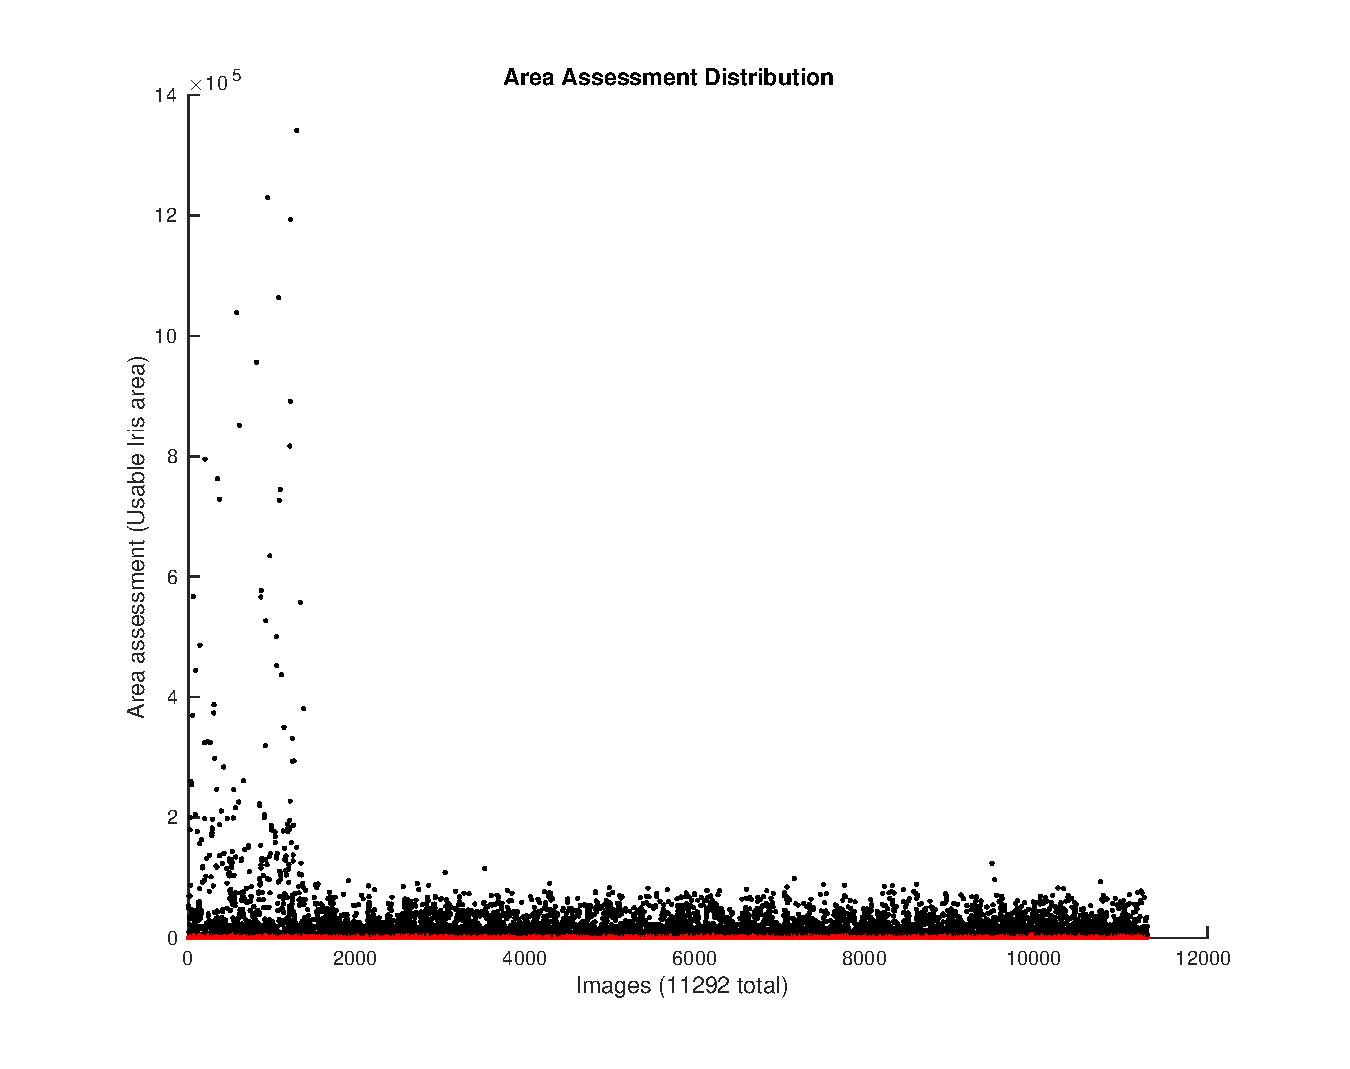
\includegraphics[height=2cm, width=5cm]{pics/dist_area_assess}
		\caption{Usable area\cite{hugo}}
		\label{fig:area}
	\end{wrapfigure}
The usable area metric is not affected by the resolution of the image and its
value is the number of pixels in the noise-free iris area.
In figure \ref{fig:area}, a clustering close to the bottom implies a
distribution weighted to the lower end of the spectrum. An higher values clearly
differing from the initial clustering.  This should mean that it is possible to
differentiate between inter-class values during classification for the metric.

\subsubsection{IQA - Iris Off-Angle Metric}\vspace{-5mm}
	\begin{wrapfigure}{R}{0.325\linewidth}
		\centering
		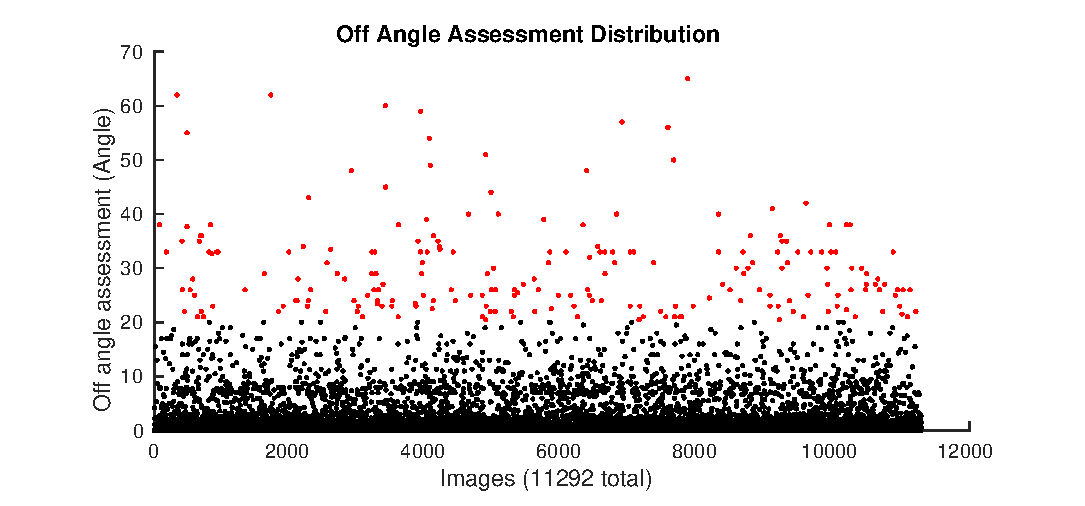
\includegraphics[height=2.25cm, width=5cm]{pics/dist_off_angle_deg_2}
		\caption{Off-angle assess. \cite{hugo}}
		\label{fig:ang}
	\end{wrapfigure}
The off-angle metric states how much the iris is rotated since a non-direct gaze
into the camera will make it oval and rotate it slightly. In figure
\ref{fig:ang} the angle lies between 0\degree and 85\degree.
5\degree-10\degree seems to be outside the normal distribution. In the figure 
angles above 20\degree has been marked as "bad" angles, because they are far
outside the normal distribution.  There is a large inter class distance which
suggests a good possibility to differentiate the metrics. 

\vspace{-5mm}
\subsubsection{IQA - Focus Metric}\vspace{-5mm}
	\begin{wrapfigure}{R}{0.325\linewidth}
		\centering
		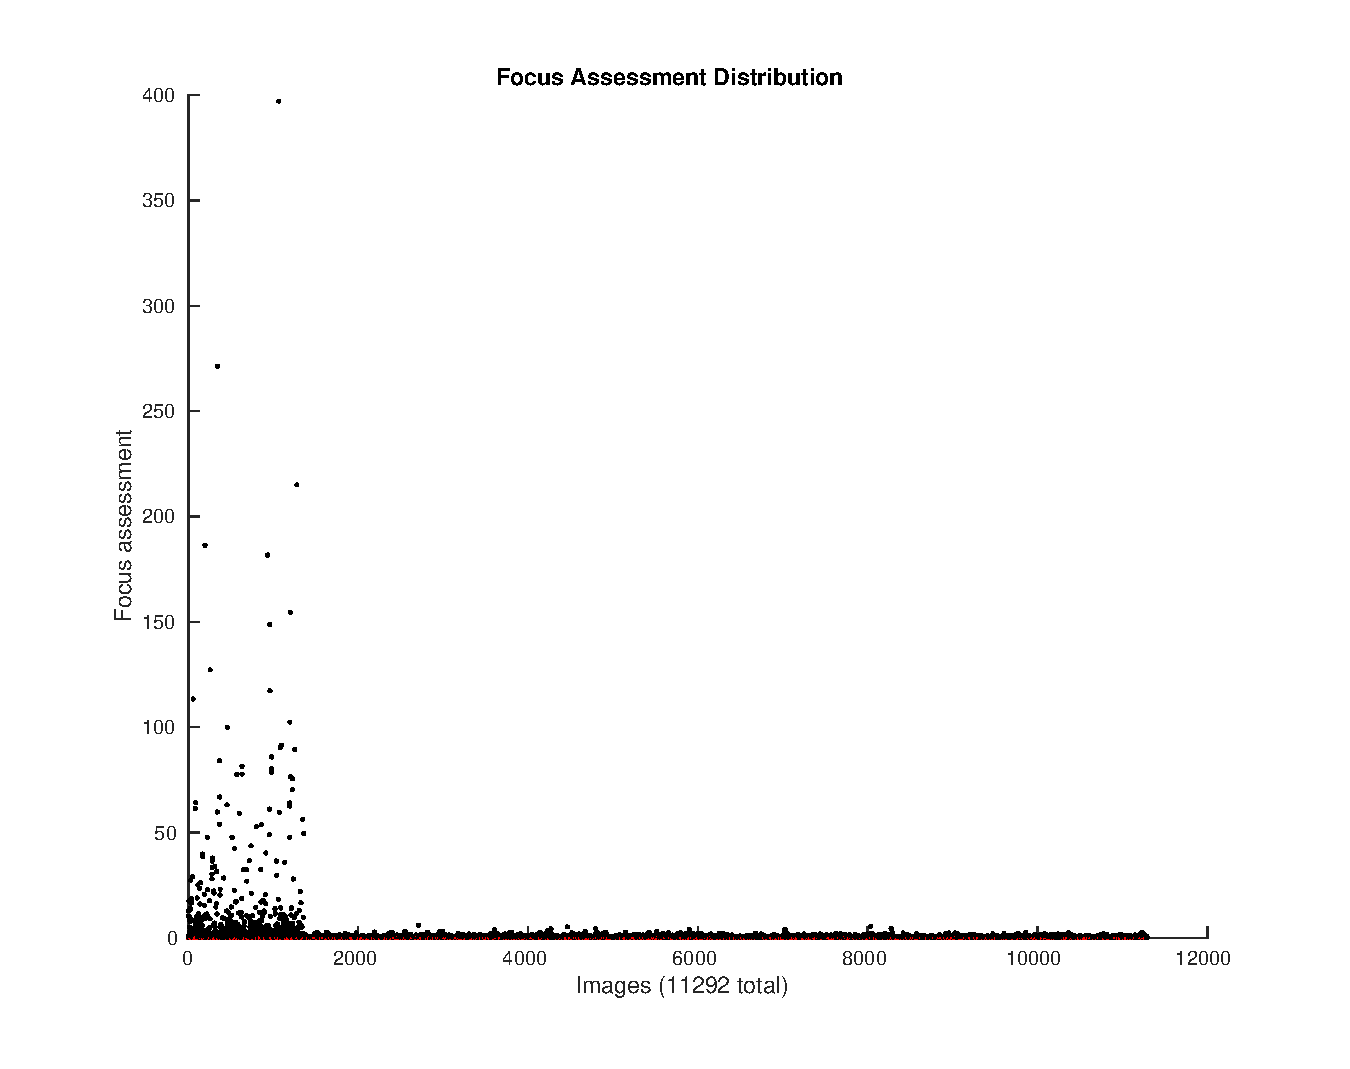
\includegraphics[height=2cm, width=5cm]{pics/dist_focus_assess}
		\caption{Focus assessment \cite{hugo}}
		\label{fig:focus} 
	\end{wrapfigure}
The focus metric is dictated by the relative magnitude to the mean value.
Because the images were not scaled to equal size some images has higher values
than the rest.  It also shows that there are images with low focus in the subset
as well.  The mean value is represented as the value 1, all values above 1 is
therefore considered to be of better focus than those below.

\vspace{-5mm}
\subsubsection{IQA - Motion Blur Metric}\vspace{-5mm}
	\begin{wrapfigure}{R}{0.325\linewidth}
		\centering
		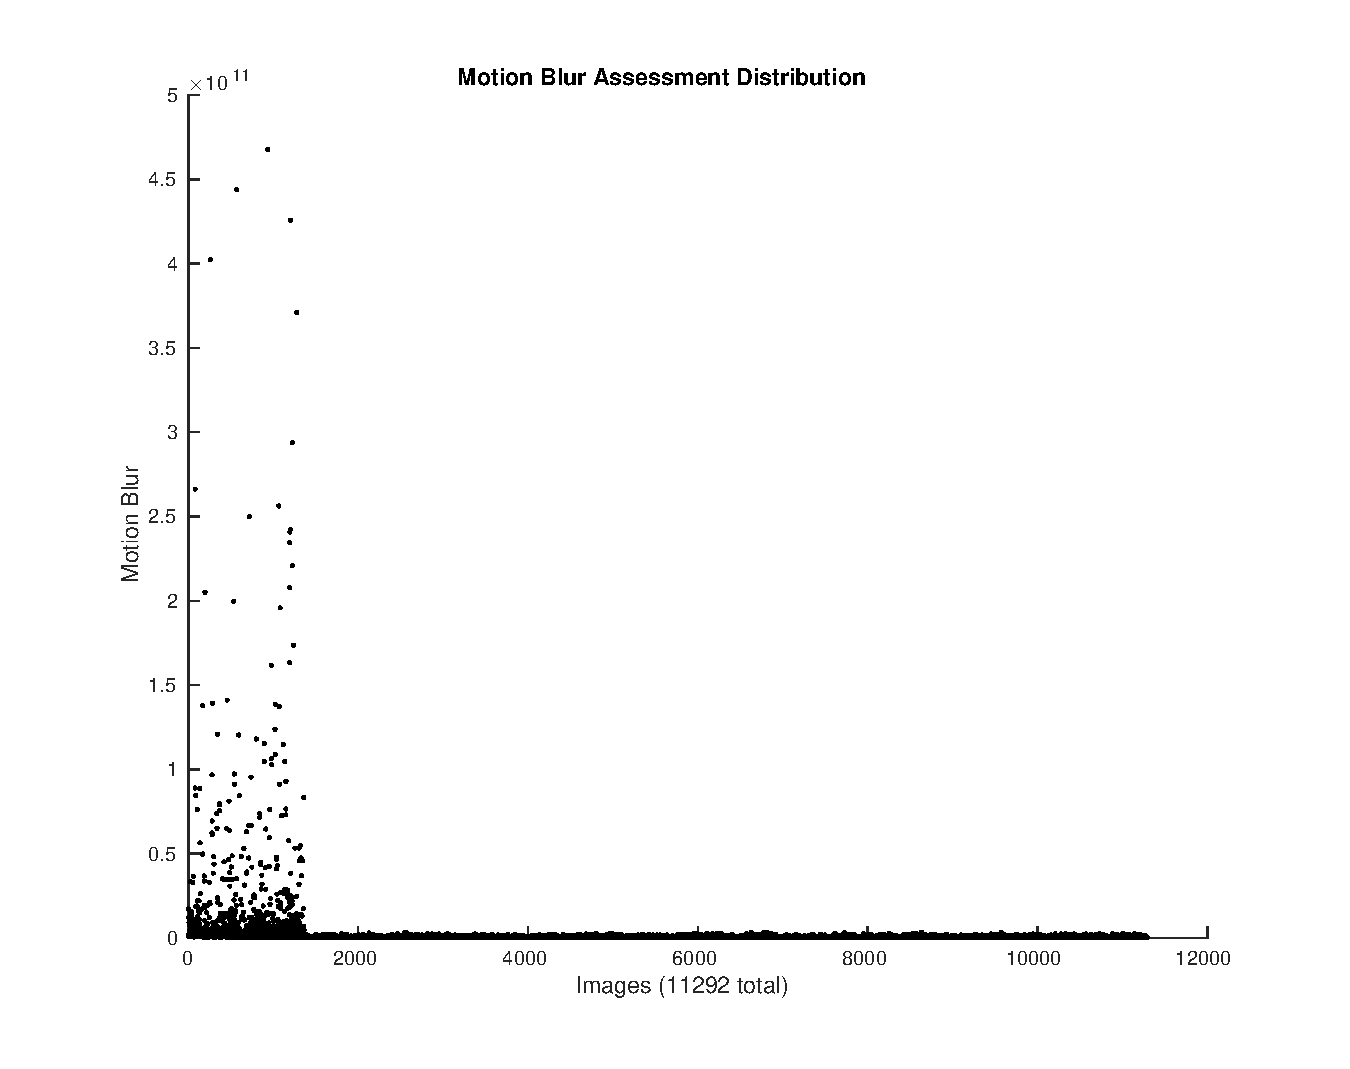
\includegraphics[height=2cm, width=5cm]{pics/dist_motion_blur_mag}
		\caption{Motion blur mag. \cite{hugo}}
		\label{fig:motion}
	\end{wrapfigure}
Motion blur is dictated by angle and magnitude of Fourier spectrum. This paper 
only evaluates the magnitude, where a higher value with more blur.
As for focus assessment, the same problem occurs for motion blur
assessment, figure \ref{fig:motion}.  The higher resolution images seems to have
much more blur than the than the UBIRIS data sets, suggesting  that the metric
may not be usable.

\vspace{-5mm}
\subsubsection{IQA - Pupil Dilation Metric}\vspace{-5mm}
	\begin{wrapfigure}{R}{0.325\linewidth}
		\centering
		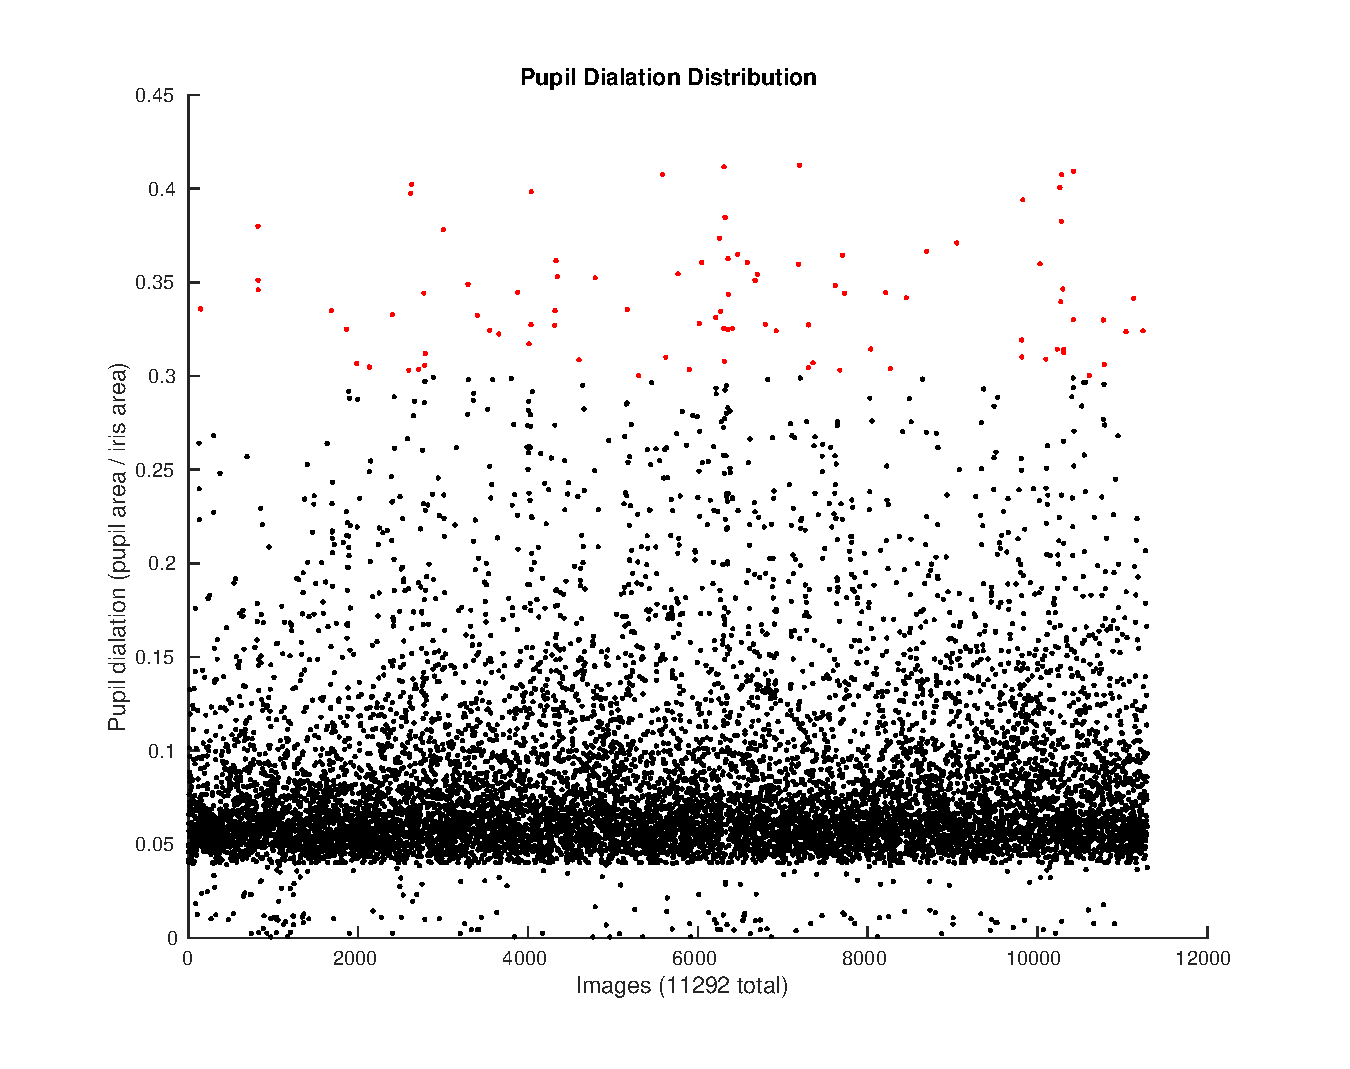
\includegraphics[height=1.5cm, width=5cm]{pics/dist_pupil_dilation_ratio}
		\caption{Pupil to iris ratio \cite{hugo}}
		\label{fig:ratio}
	\end{wrapfigure}
Figure \ref{fig:ratio} shows a very clear normal distribution which is equal
for all images.  This suggests that there is a good chance of performing
classification on this metric. This is however not likely because during
classification, the pupils where not distinctively larger for bad images.



\clearpage
\subsection{BIQA Metric analysis}
\vspace{-3mm}
\subsubsection{BIQA - Usable Iris Area Metric}\vspace{-5mm}
	\begin{wrapfigure}{R}{0.325\linewidth}
		\centering
		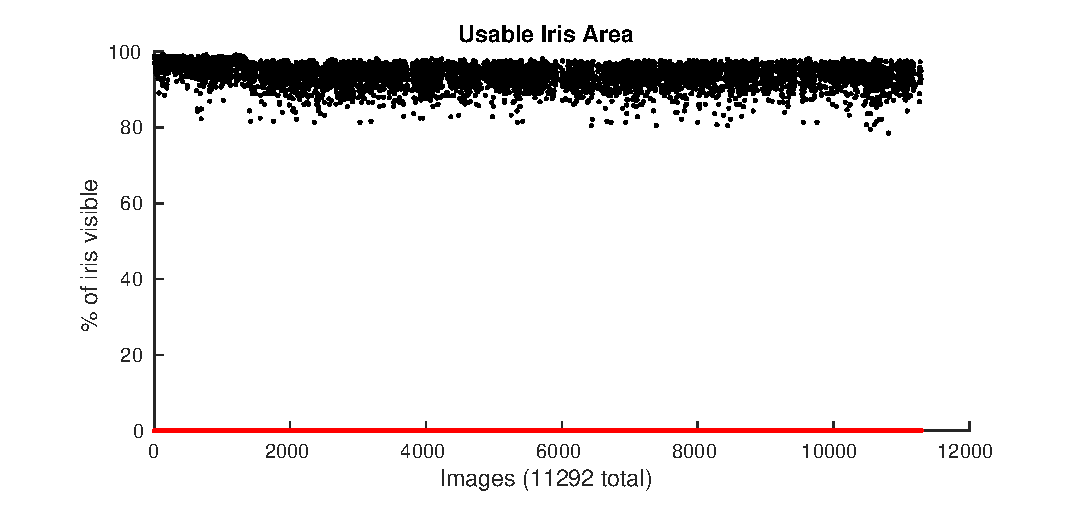
\includegraphics[height=2.25cm, width=5cm]{pics/biqa_dist_uia}
		\caption{Usable iris area \cite{iso}}
		\label{fig:uia}
	\end{wrapfigure}
The usable area metric differs from pupil dilation metric by incorporating
occlusions. This project did not implement this, meaning it is almost equal to
the pupil dilation metric.  This metric is the iris area minus the pupil area.
In figure \ref{fig:uia}, one can see that all the images is clustered to the top
which has a tight grouping making it hard to differentiate. Except for the
images which was unable to retrieve the metric from.


\vspace{-5mm}
\subsubsection{BIQA - Pupil-Iris Contrast Metric}\vspace{-5mm}
	\begin{wrapfigure}{R}{0.325\linewidth}
		\centering
		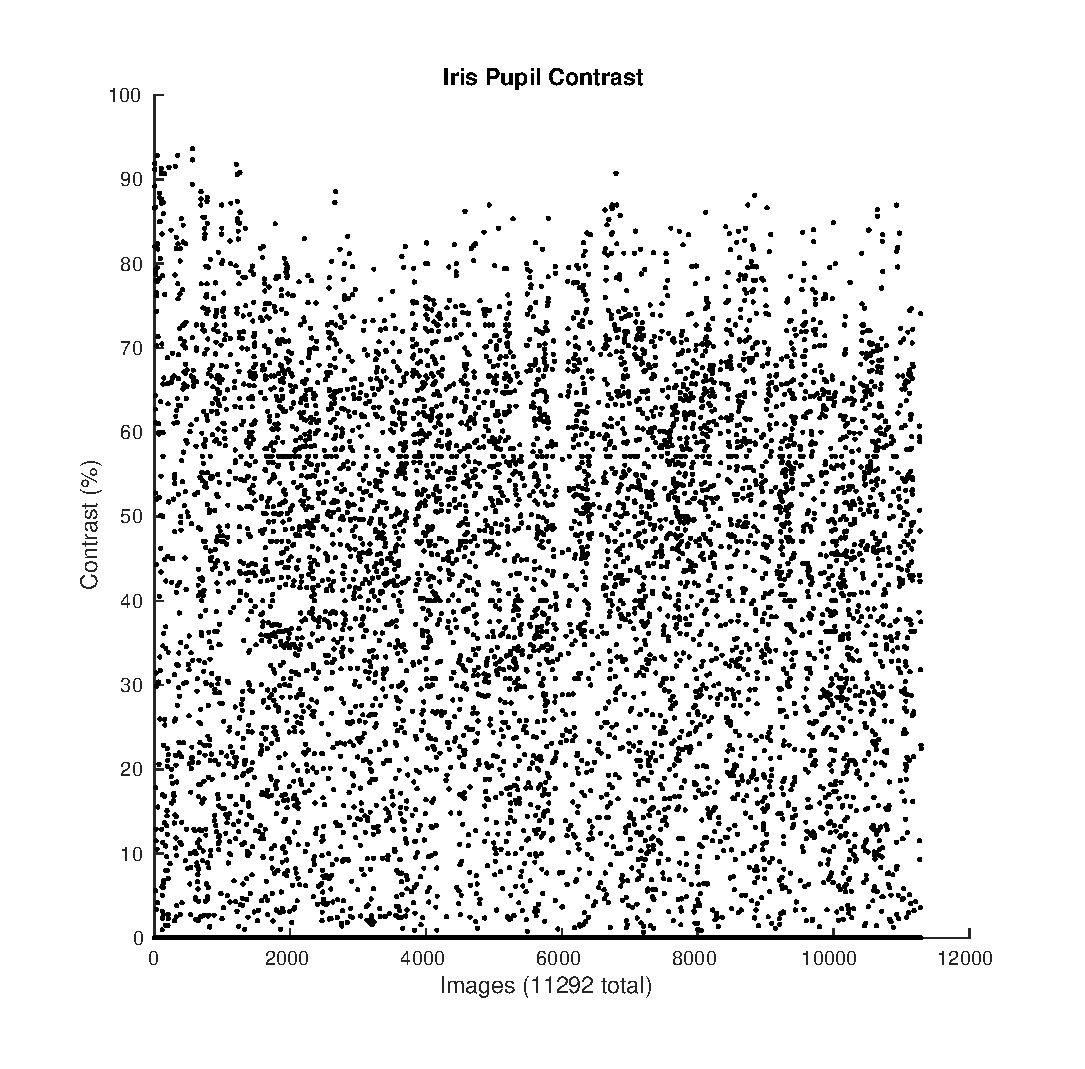
\includegraphics[height=1.25cm, width=5cm]{pics/biqa_dist_ipc}
		\caption{Pupil-iris contrast \cite{iso}}
		\label{fig:ipc}
	\end{wrapfigure}
The ISO standard sets forth the metric of pupil-to-iris contrast. In figure
\ref{fig:ipc}, one can see that this value is sparsely spread out. This could
state that there is a separation between different types of irises, or that
there is no definitive patterns to classify by.


\vspace{-5mm}
\subsubsection{BIQA - Iris-Sclera Contrast Metric}\vspace{-5mm}
	\begin{wrapfigure}{R}{0.325\linewidth}
		\centering
		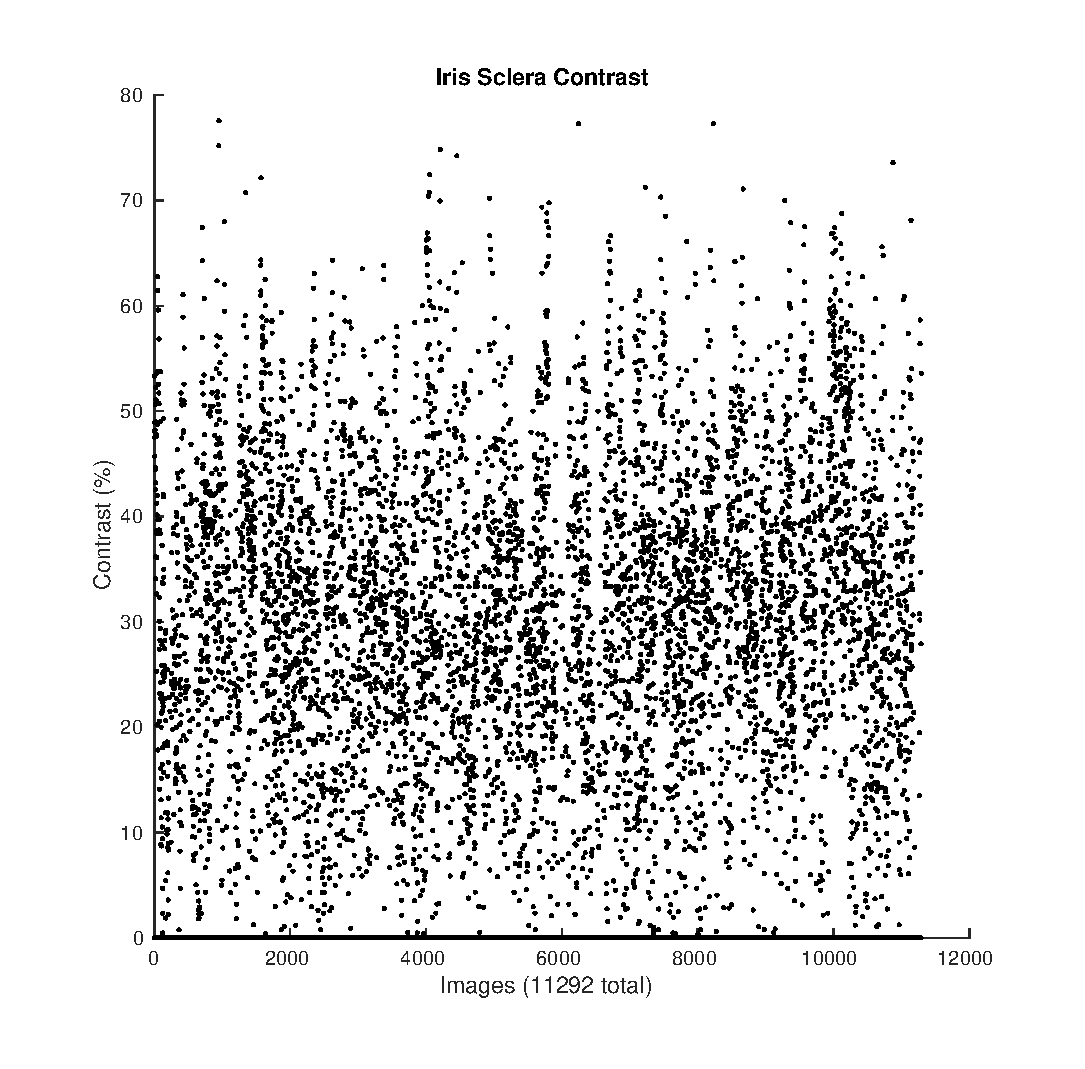
\includegraphics[height=1.25cm, width=5cm]{pics/biqa_dist_isc}
		\caption{Iris-sclera \cite{iso}}
		\label{fig:isc}
	\end{wrapfigure}
The ISO standard sets forth the metric of iris-to-sclera contrast. In figure
\ref{fig:isc}, one can see that this value is sparsely spread out. Just like the
iris-to-pupil contrast.  This could also  mean that is or is not at separation
that divides the different intra class types of contrasts.


\vspace{-5mm}
\subsubsection{BIQA - Pupil/Iris Ratio Metric}\vspace{-5mm}
	\begin{wrapfigure}{R}{0.325\linewidth}
		\centering
		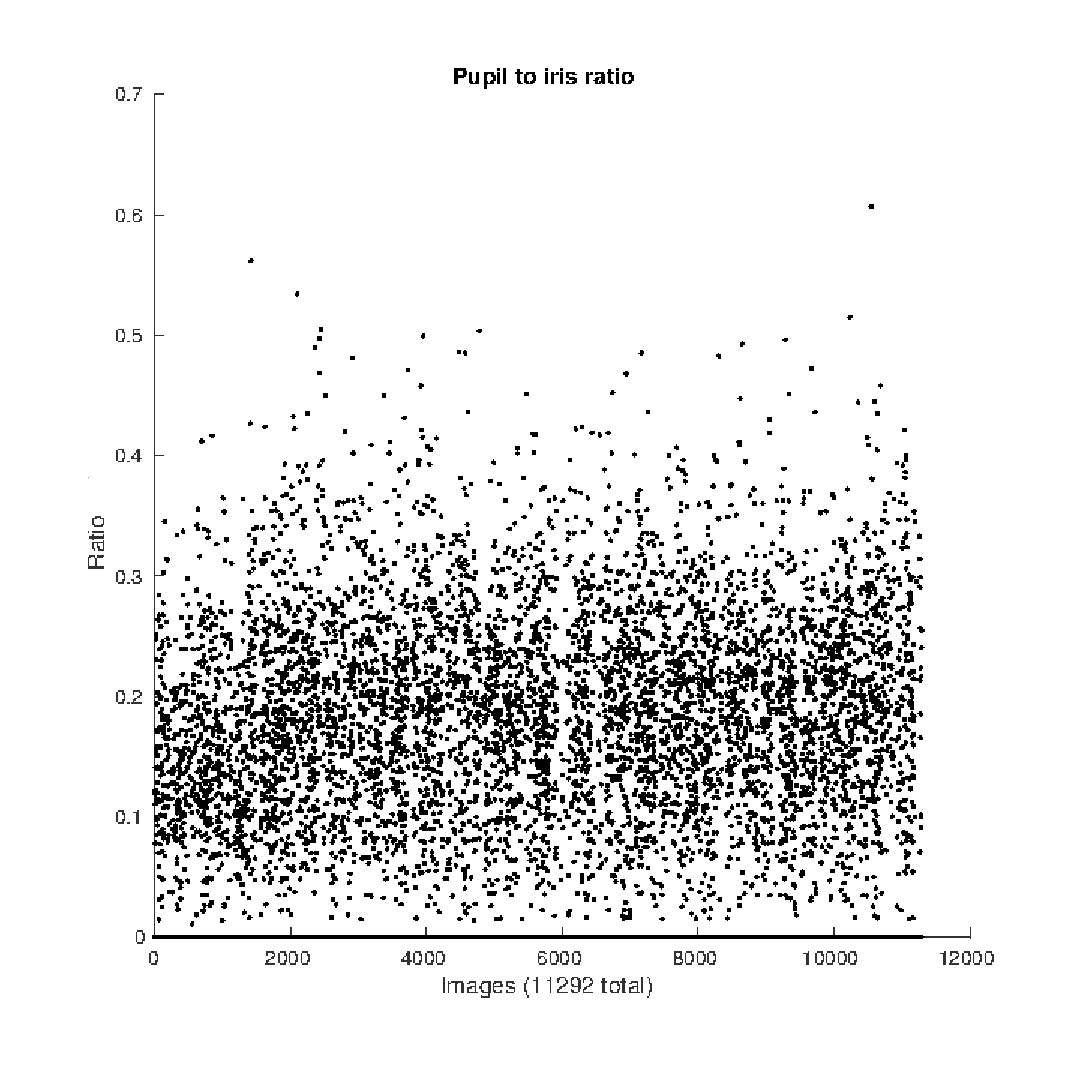
\includegraphics[height=1.25cm, width=5cm]{pics/biqa_dist_pup_ir_ratio}
		\caption{Pupil-iris ratio \cite{iso}}
		\label{fig:pir}
	\end{wrapfigure}
The ISO standard dictates this calculation.  As seen in figure \ref{fig:pir} 
there is a uniform distribution which appears to be loosely scattered throughout
the data sets.  It is however somewhat centralised around 0.1 and 0.2, but not
very distinctively.


\vspace{-5mm}
\subsubsection{BIQA - Grey Scale Utilisation Metric}\vspace{-5mm}
	\begin{wrapfigure}{R}{0.325\linewidth}
		\centering
		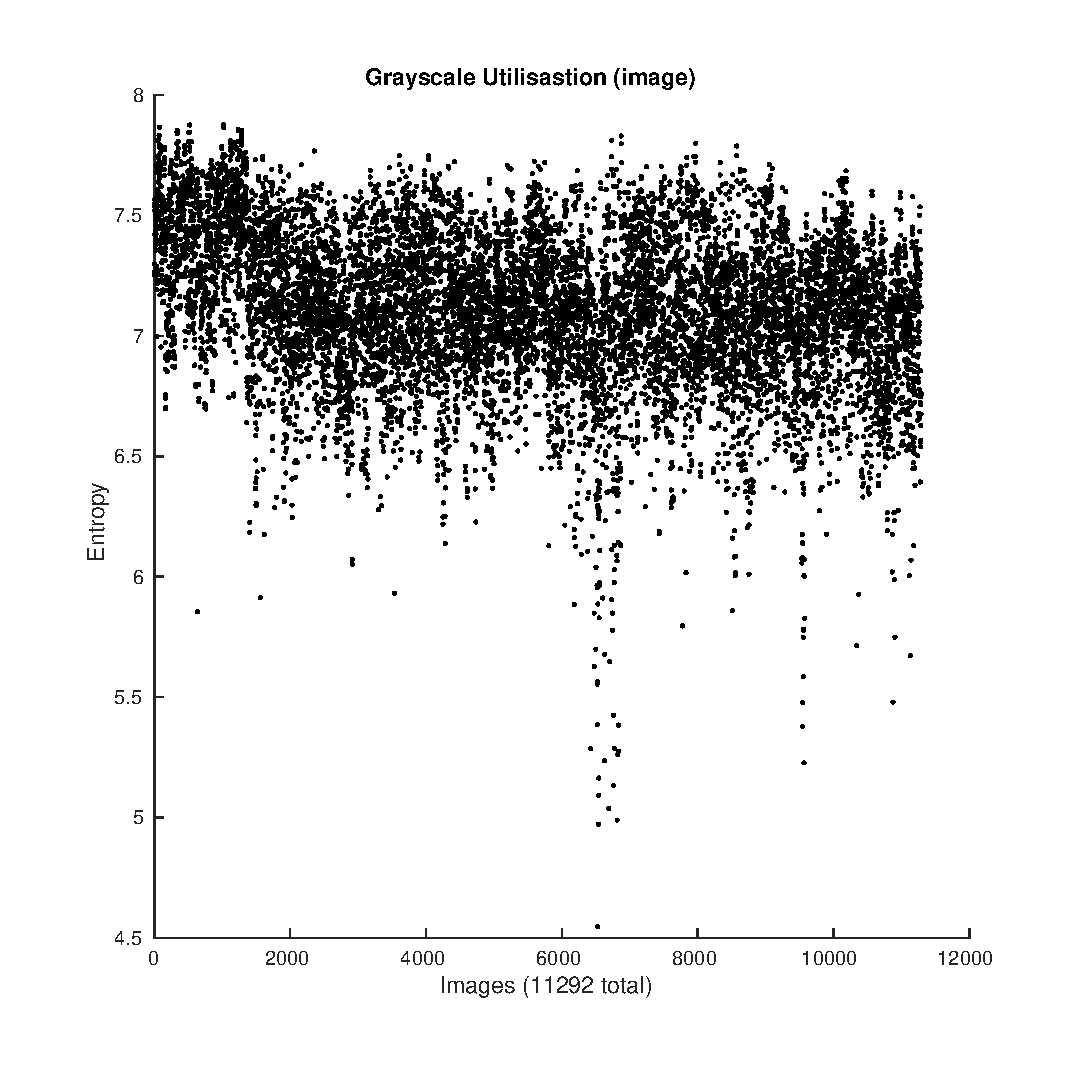
\includegraphics[height=2cm, width=5cm]{pics/biqa_dist_gsu_full}
		\caption{GSU of image \cite{iso}}
		\label{fig:gsuf}
	\end{wrapfigure}
As described in the previous sections GSU is calculated as the entropy of the
grey scale values that occur in a section or the entire image.  As seen in figure
\ref{fig:gsuf}, the distribution is equal to a normal distribution.  It also
shows that there are images with higher entropy than the rest, especially the
NTNU and MICHE data sets.  It also clearly shows images with lower entropy than
the rest.


\vspace{-5mm}
\subsubsection{BIQA - NIQE Metric}\vspace{-5mm}
	\begin{wrapfigure}{R}{0.325\linewidth}
		\centering
		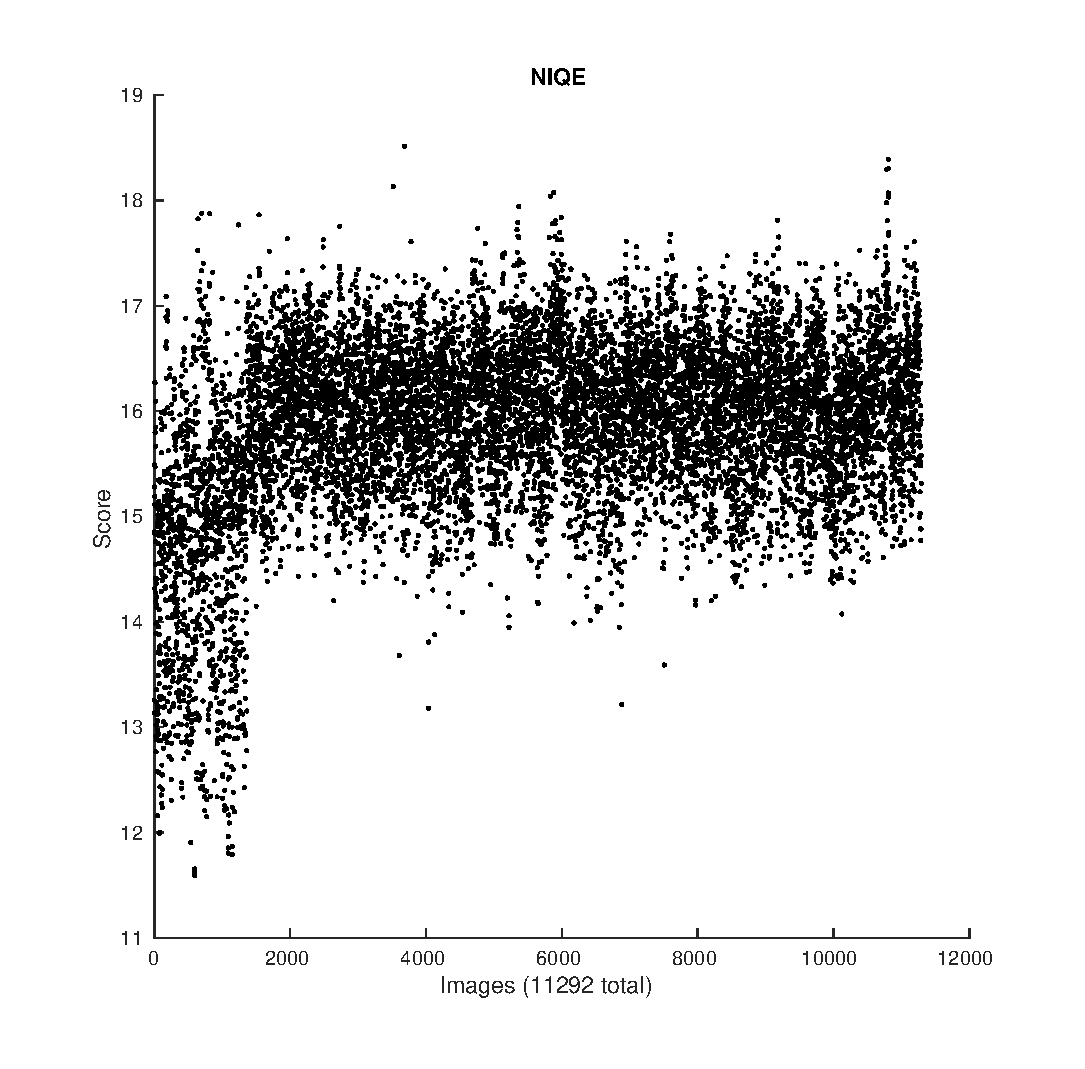
\includegraphics[height=2cm, width=5cm]{pics/biqa_dist_niqe}
		\caption{NIQE alg \cite{niqe}}
		\label{fig:niqe}
	\end{wrapfigure}
Anish Mittal et. al developed Natural Image Quality Evaluator (NIQE), a blind 
image quality model\cite{niqe}.  It assesses the image based on natural scene
statistics (NSS) as explained by L. Ruderman\cite{nss}.
In this model the resulting quality metric is described as the lower values
dictate better natural scene statistics. Therefore higher quality value is
related to a lower output value from NIQE.

Given this statistic, a method for performing classification should be very
possible, but as seen in figure \ref{fig:niqe} a distinct singular value
separating the system does not appear directly.  However one can see that there
are a quite normal distribution where the outliers represent certain images that
are of much higher quality and lower quality.


\vspace{-5mm}
\subsubsection{BIQA - BRISQUE Metric}\vspace{-5mm}
	\begin{wrapfigure}{R}{0.325\linewidth}
		\centering
		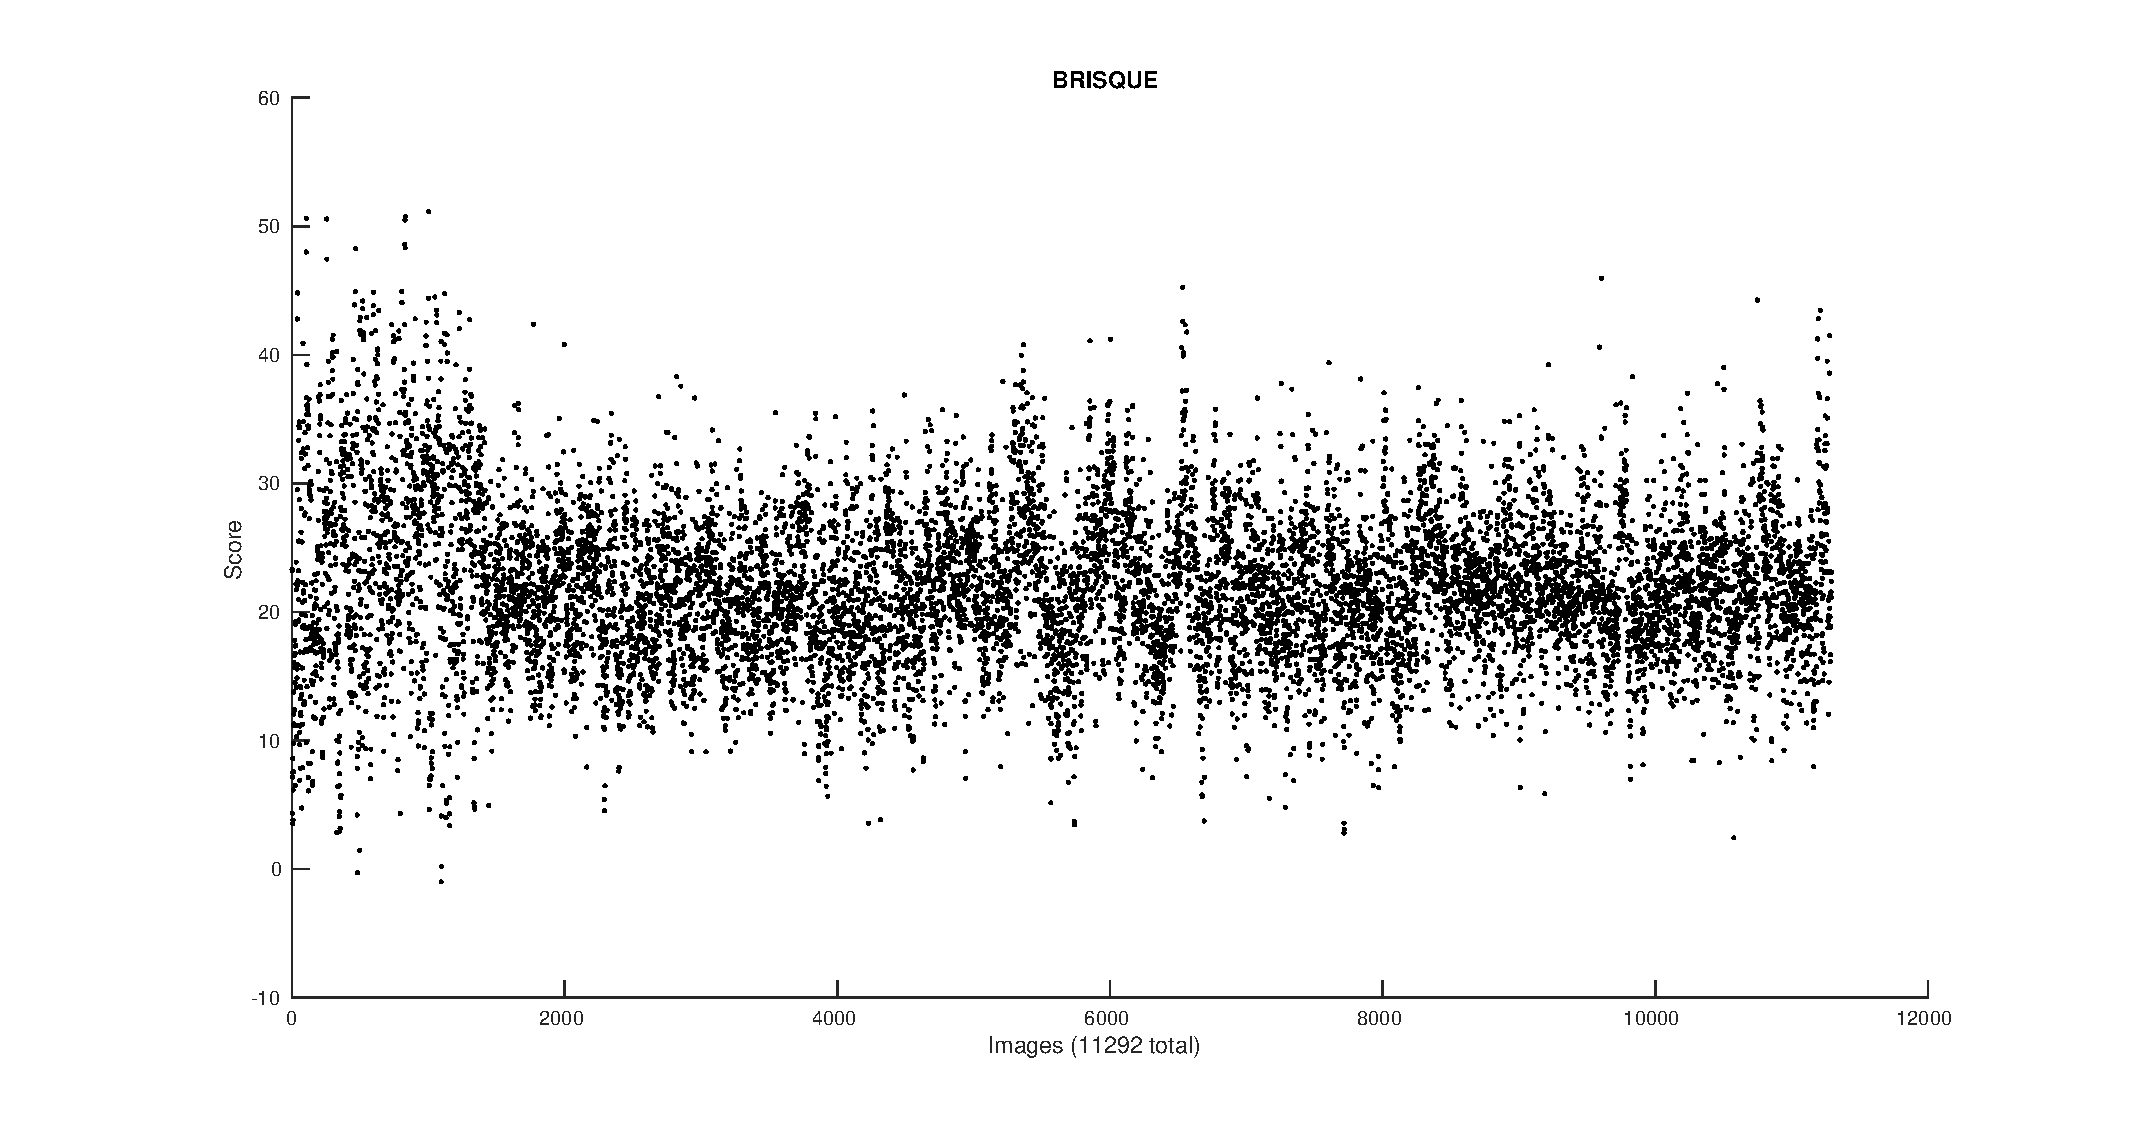
\includegraphics[height=2.25cm, width=5cm]{pics/biqa_dist_brisque}
		\caption{BRISQUE alg \cite{brisque}}
		\label{fig:brisque}
	\end{wrapfigure}
The BRISQUE metric is calculated by the tool developed by Anish Mittal et.
al\cite{brisque}. They have developed a blind image quality assessment model
operating in the spacial domain.  As with NIQE, BRISQUE also focuses on the use
of scene statistics to quantify the quality.  It evaluates the possible loss of
"naturalness".
As with many of the others metrics, there is a clear normal distribution as
well. Images that are of better quality, has a lower metric value than those of
inferior quality.


\vspace{-5mm}
\subsubsection{BIQA - JP2KNR Metric}\vspace{-5mm}
	\begin{wrapfigure}{R}{0.325\linewidth}
		\centering
		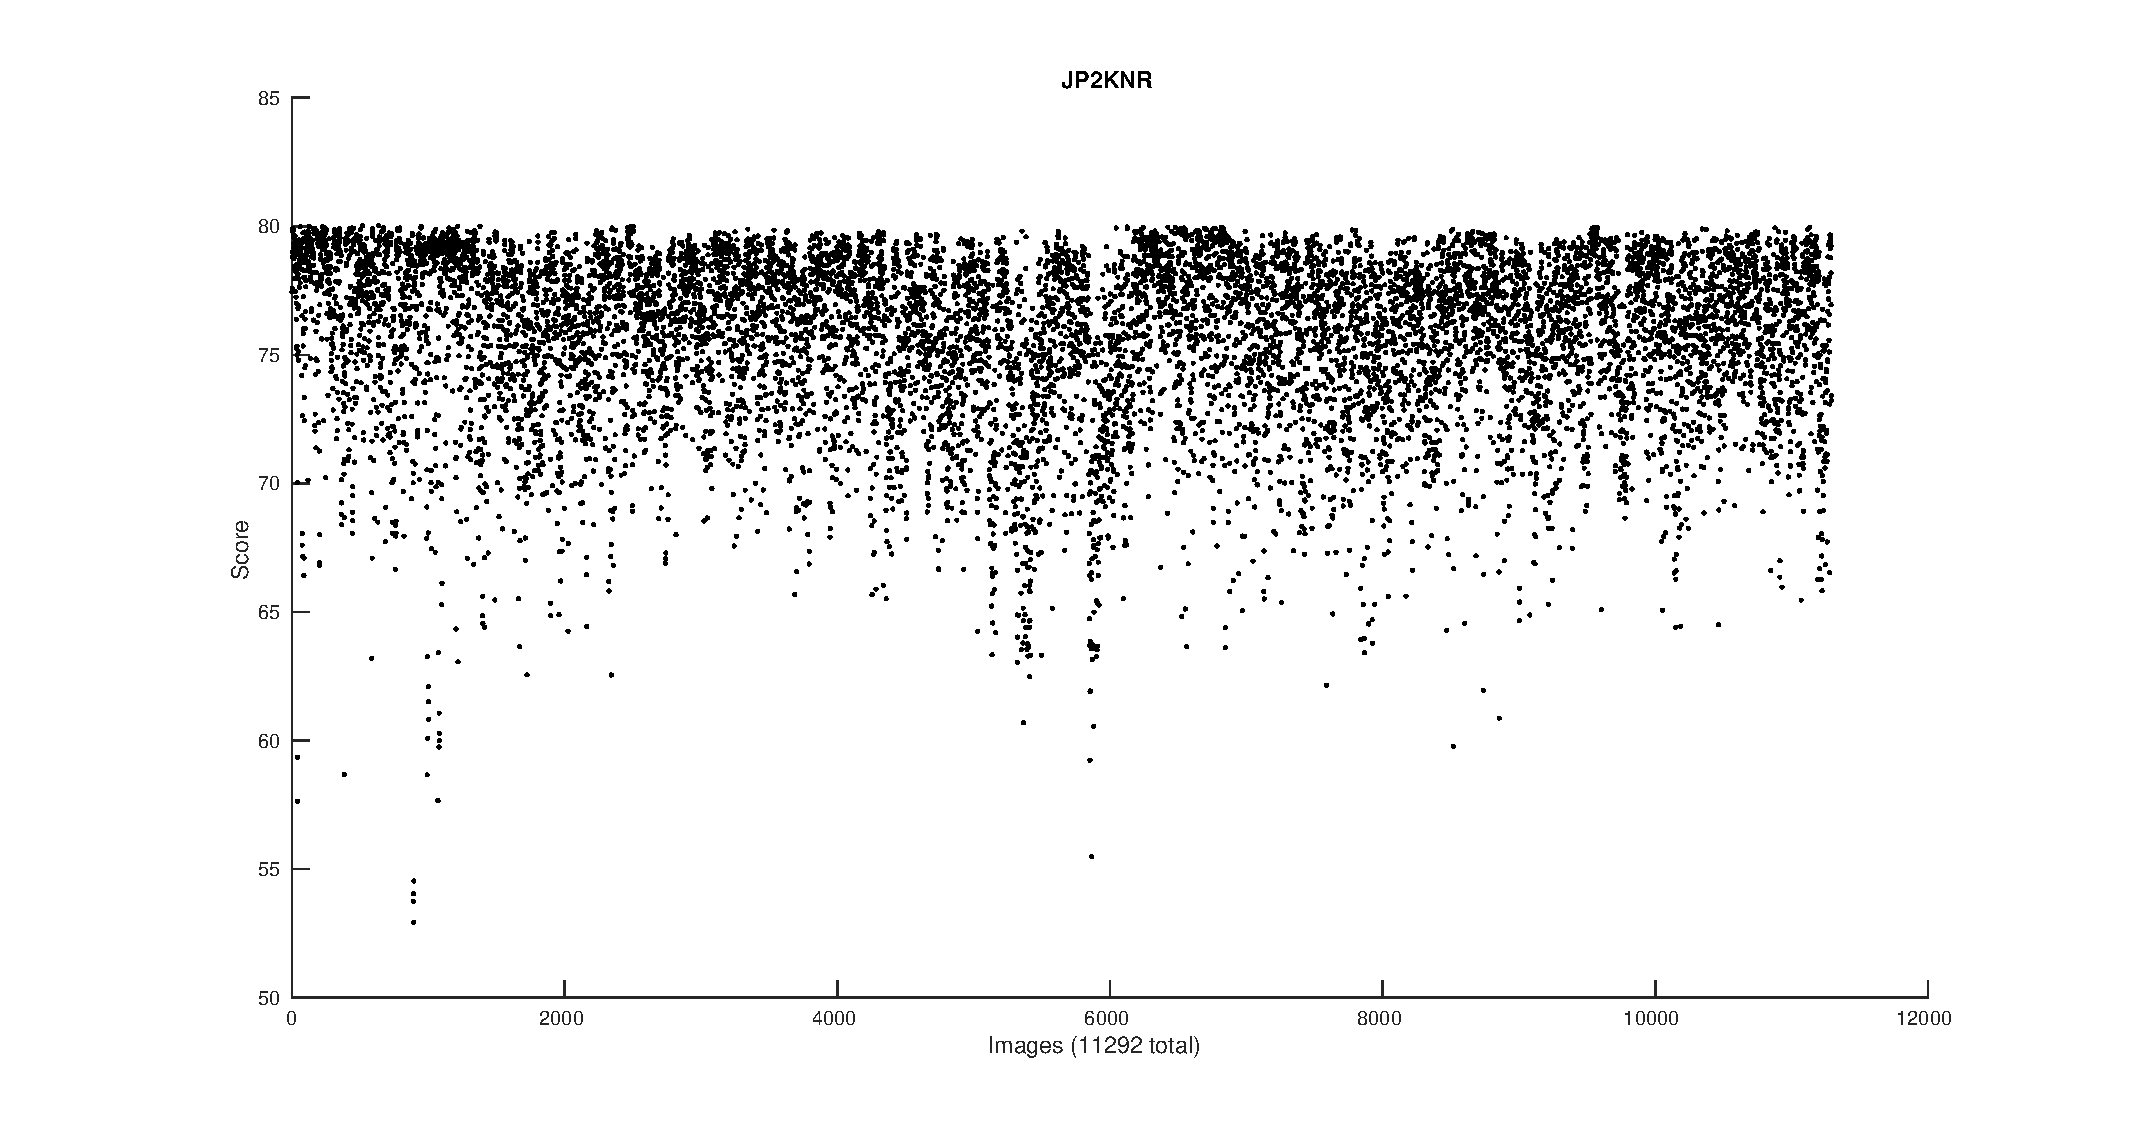
\includegraphics[height=2.75cm, width=5cm]{pics/biqa_dist_jp2knr}
		\caption{JP2KNR alg \cite{jp2knr}}
		\label{fig:jp2knr}
	\end{wrapfigure}
Hamid R. Sheikh et. al created the JP2KNR tool, which employs a method of
applying natural scene statistics to measure quality of images that has been
compressed using wavelet compression.  It seeks to quantify the the loss of
quality which can be related to the human perception of quality.
As opposed to BRISQUE and NIQE, JP2KNRs metric value states that a higher value
is equal to higher quality and low metric value is equal to a lower metric
value.
As shown in figure \ref{fig:jp2knr}, there is a distinct value of the images
with a quite clear maximum level of quality.  This gives the distribution of a
peak positioned to the far right-side of the graph.


\vspace{-5mm}
\subsubsection{BIQA - BIQI Metric}\vspace{-5mm}
	\begin{wrapfigure}{R}{0.325\linewidth}
		\centering
		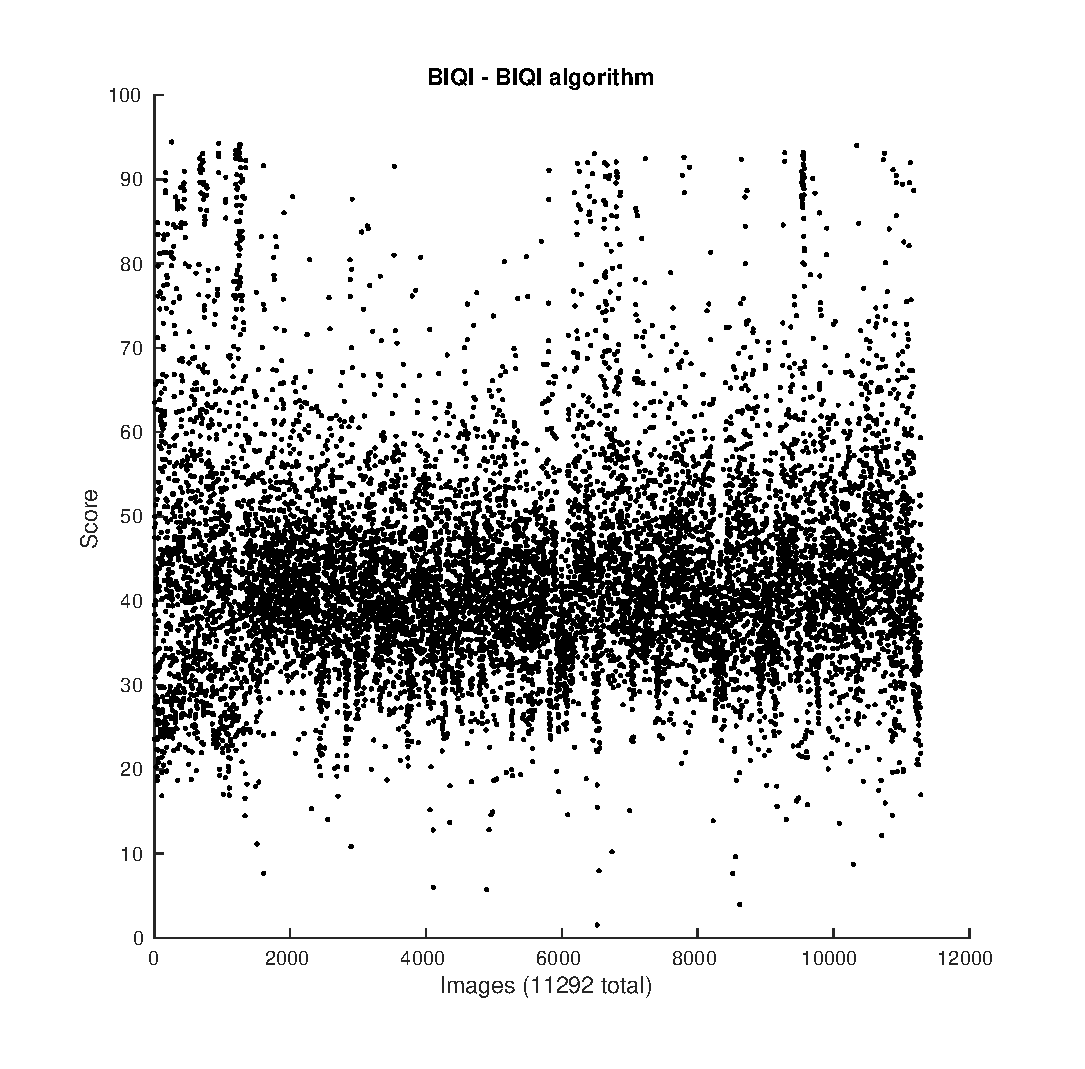
\includegraphics[height=2.75cm, width=5cm]{pics/biqa_dist_biqi_alg}
		\caption{BIQI alg \cite{biqi}}
		\label{fig:biqialg}
	\end{wrapfigure}
"Blind Image Quality Index", BIQI\cite{biqi} was developed by Anush K. Moorthy
et. al and focused on assessing the distortions of the image.  BIQI is based on
a pre-trained classifier that can be used to assess any distortion, and it is
also based on NSS.
The distribution is not as clear as with many of the other data sets, but has a
centralised distribution between 35-50 for the UBIRISv2 data set. The NTNU and
MICHE data sets does not seem to have any centralised distribution.
BIQI may therefore be unsuitable for classification.


\subsection{Classification}
After performing the classification on each of the selected metrics separately,
several of them where shown to be unable to classify the images evenly.  Even
though the training set was slightly overfitted for "good" images.

As one can see several of the metrics performed poorly, either classifying
falsely or not at all.  The IQA pupil dilation metric (fig. \ref{fig:clas_pd}),
IQA iris area (fig. \ref{fig:clas_ia}), IQA usable iris (fig. \ref{fig:clas_ua})
IQA focus assessment (fig. \ref{fig:clas_f}) and IQA motion magnitude metric
(fig. \ref{fig:clas_mot}), performed very poorly.  The pupil dilation metric are
unable to classify any as "good", while usable iris area, classifies them
with 0\%\ as "good images", and iris area classifies a few as "good".

Table \ref{tab:indclas} summarises the number classification made by the support
vector machine (SVM) after being trained with 625 "good" images and 560 "bad"
images which was manually classified with WebIIC\cite{webiic}.

\begin{figure}[h]
	\begin{minipage}{0.48\linewidth}
		\centering
		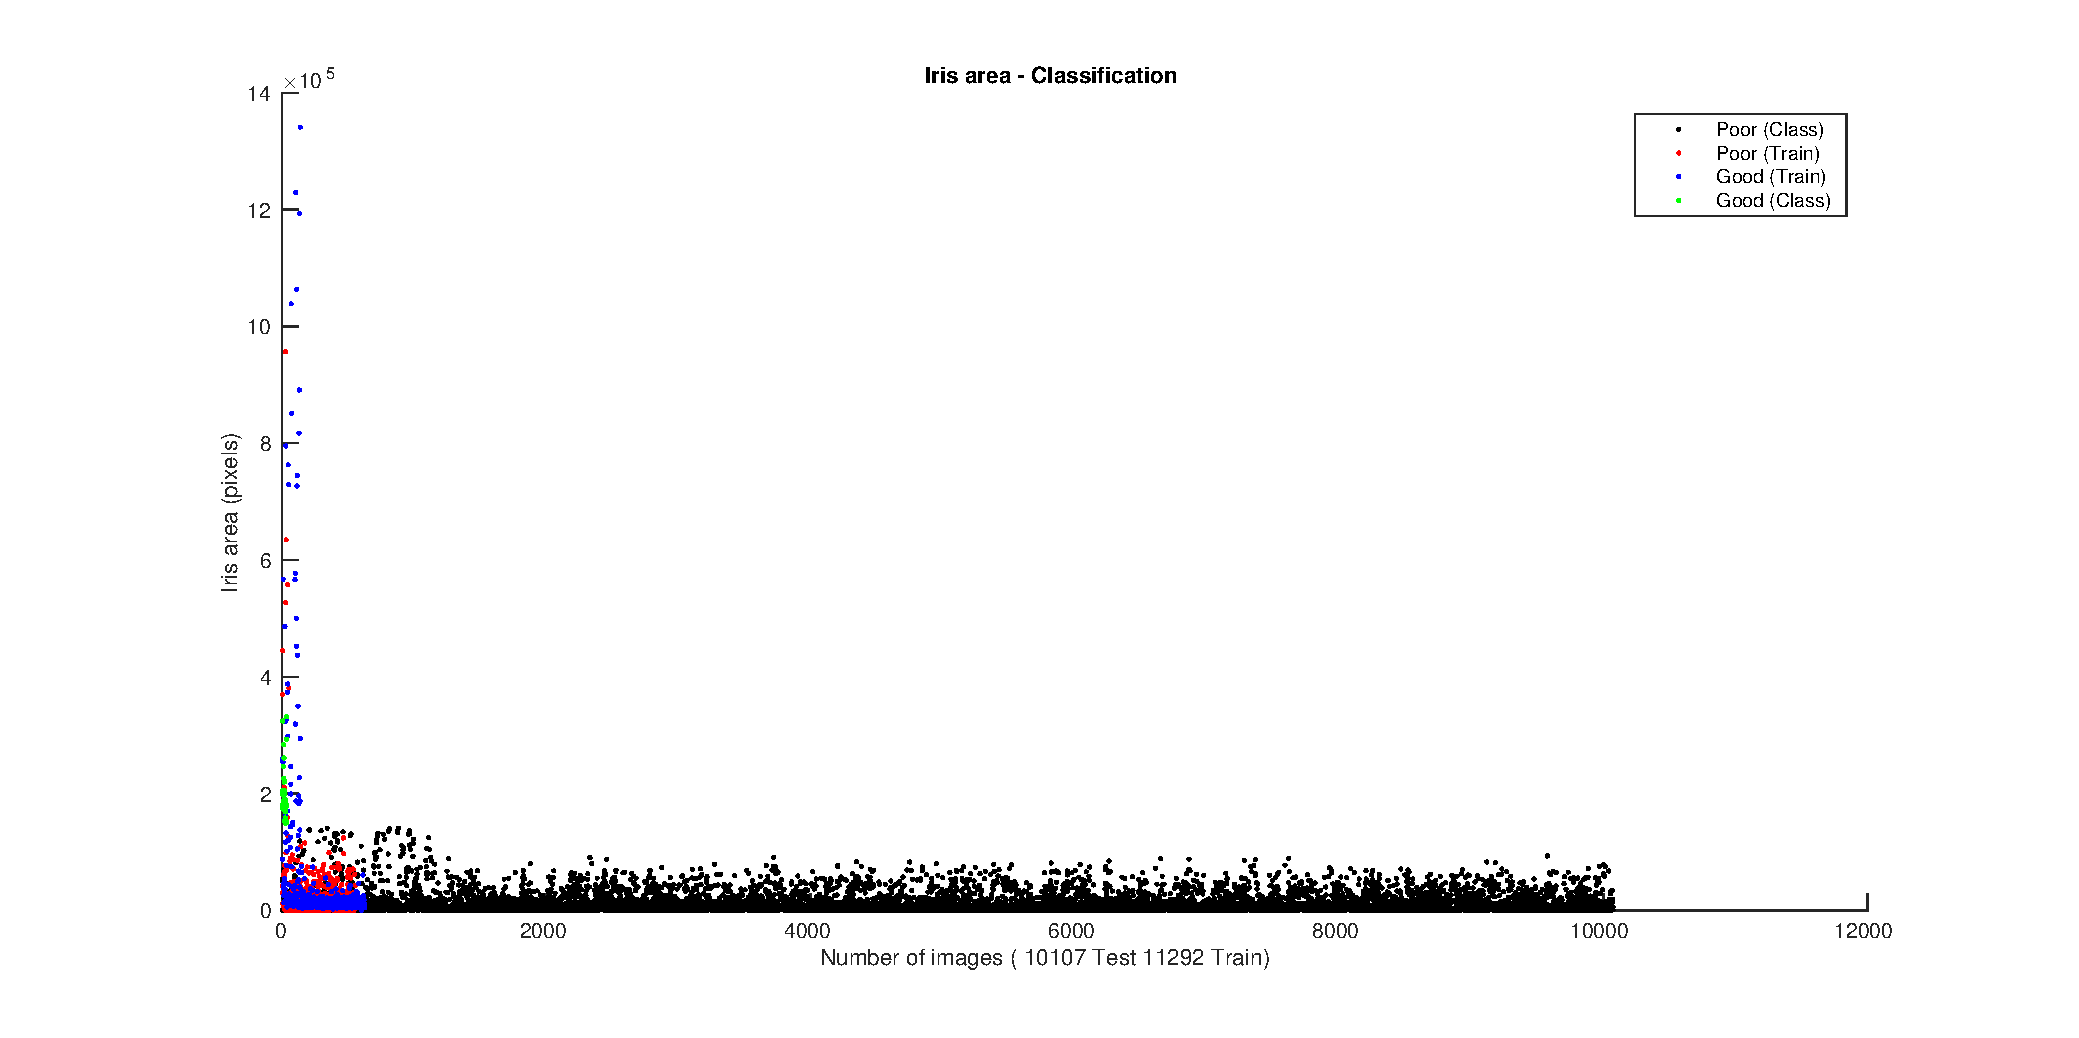
\includegraphics[width=0.9\linewidth, height=1.6cm]{pics/iqa_clas_area}
		\caption{Res. of class. using IQA iris area}
		\label{fig:clas_ia}
	\end{minipage}
	\hfill
	\begin{minipage}{0.48\linewidth}
		\centering
		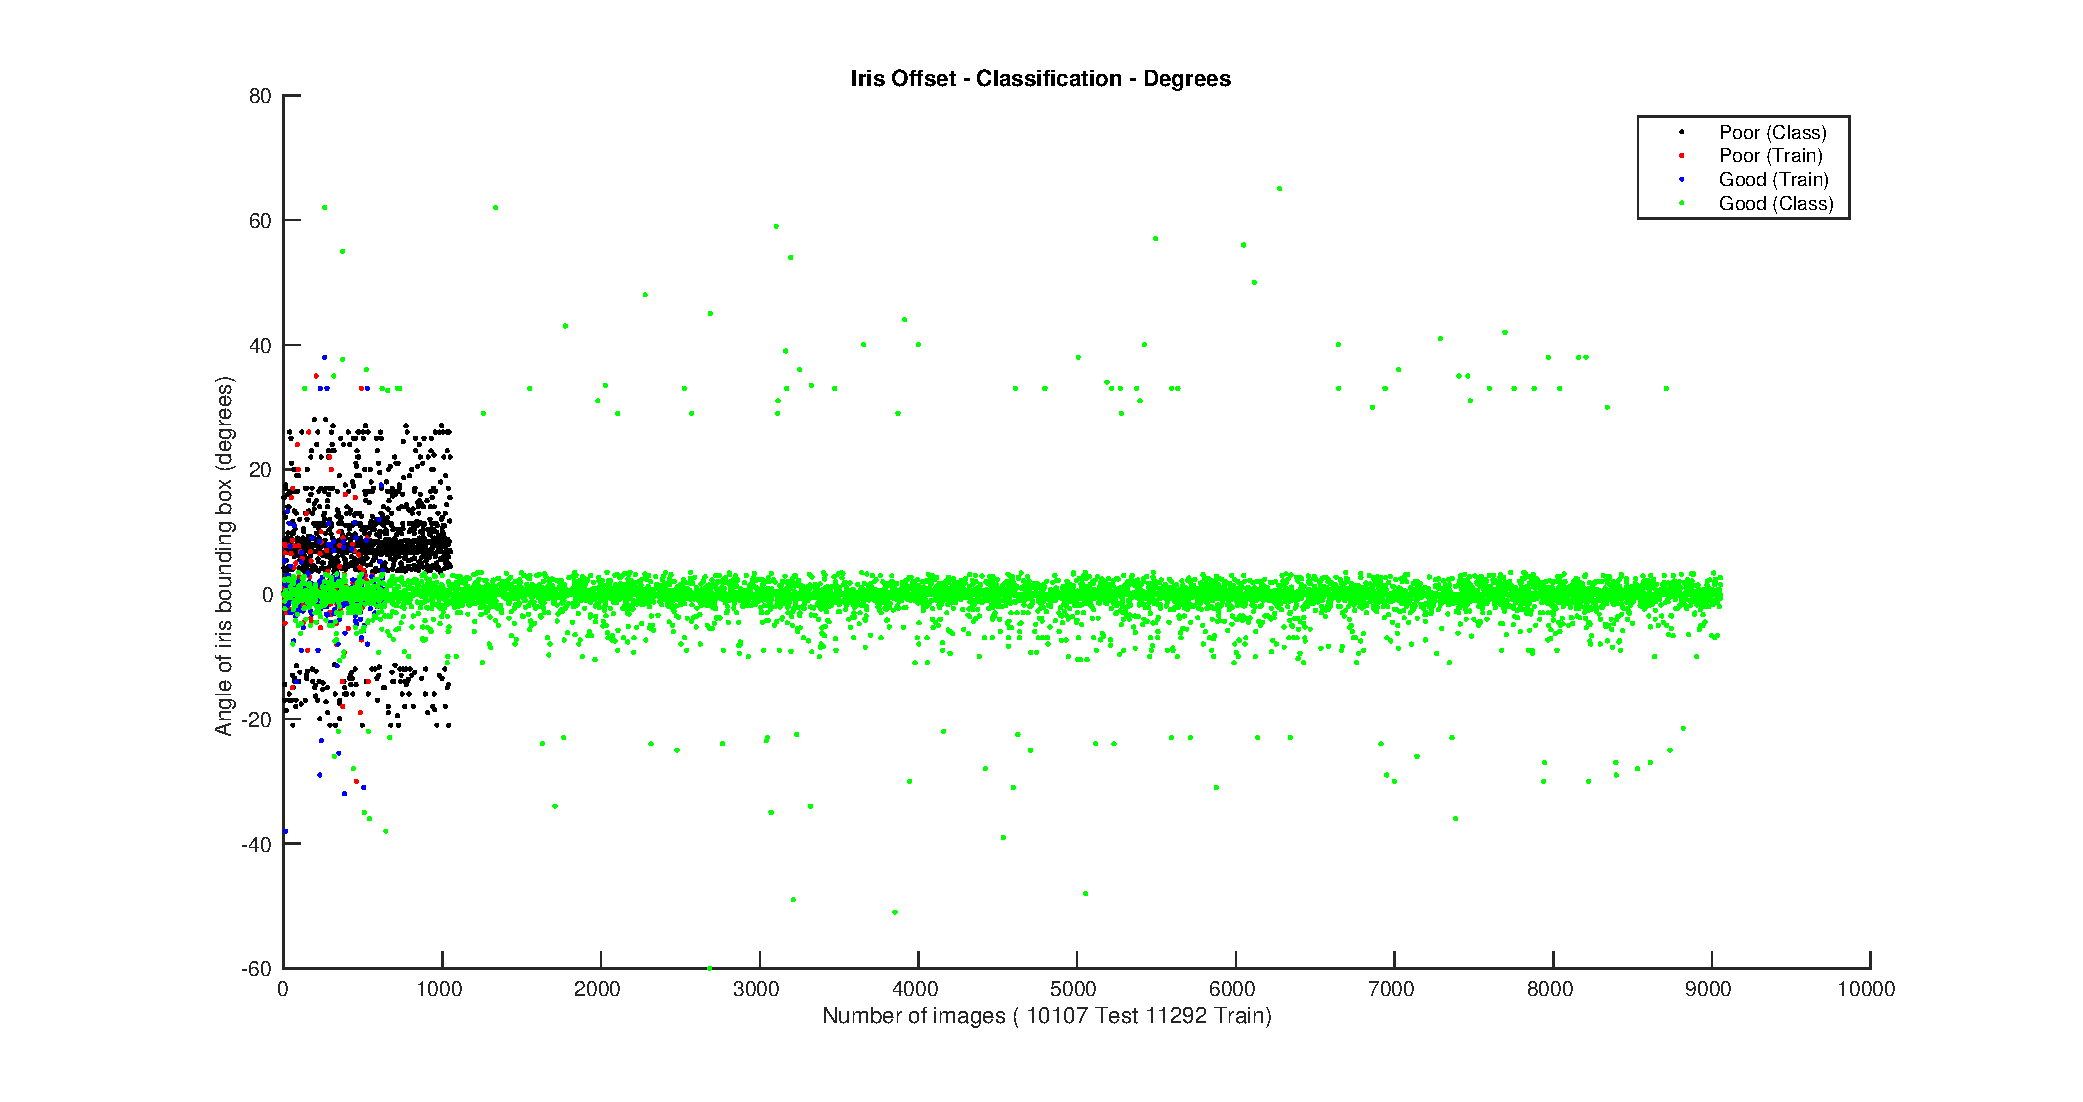
\includegraphics[width=0.9\linewidth, height=1.6cm]{pics/iqa_clas_iris_angle}
		\caption{Res. of class. using IQA iris angle}
		\label{fig:clas_ang}
	\end{minipage}
	\begin{minipage}{0.48\linewidth}
		\centering
		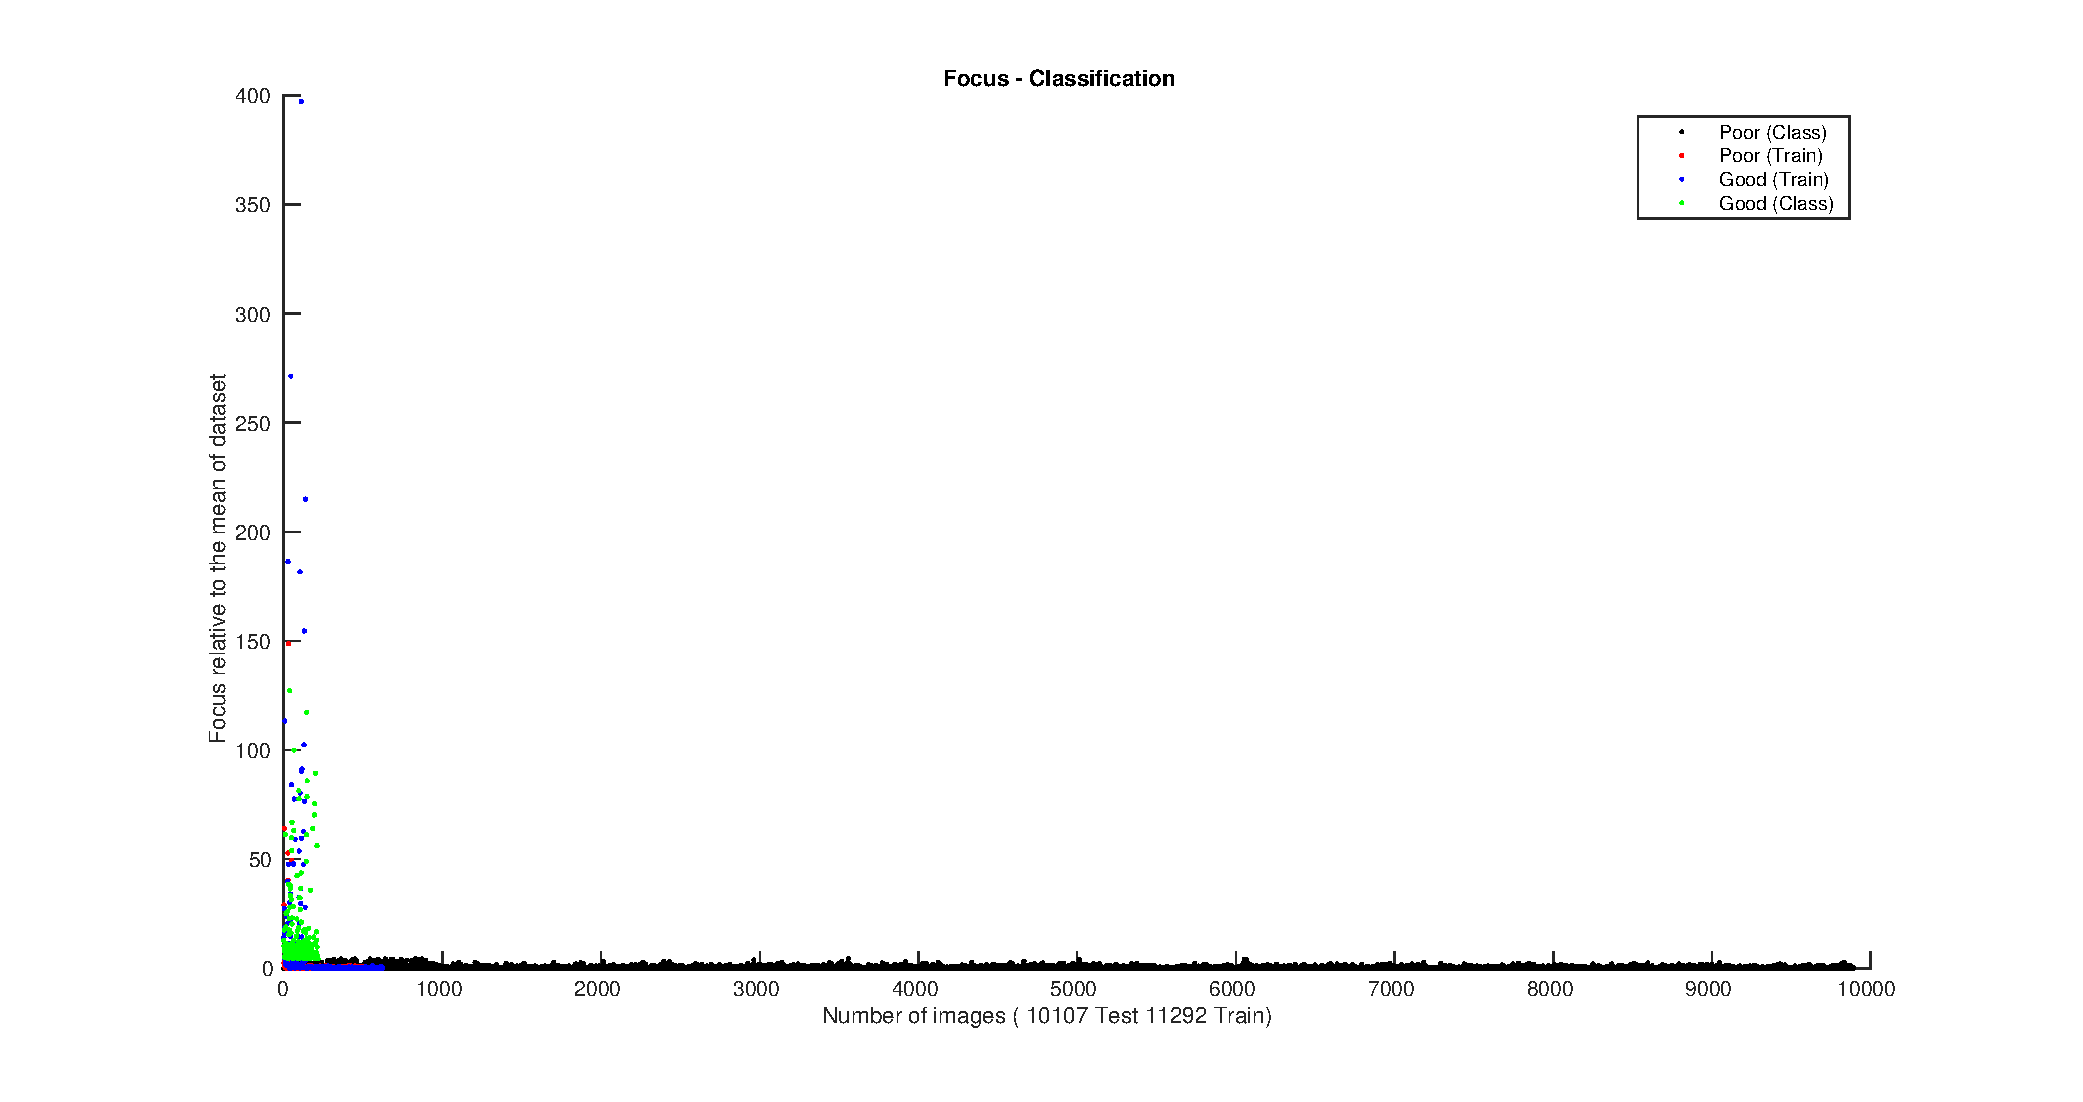
\includegraphics[width=0.9\linewidth, height=1.6cm]{pics/iqa_clas_focus}
		\caption{Res. of class. using IQA focus}
		\label{fig:clas_f}
	\end{minipage}
	\hfill
	\begin{minipage}{0.48\linewidth}
		\centering
		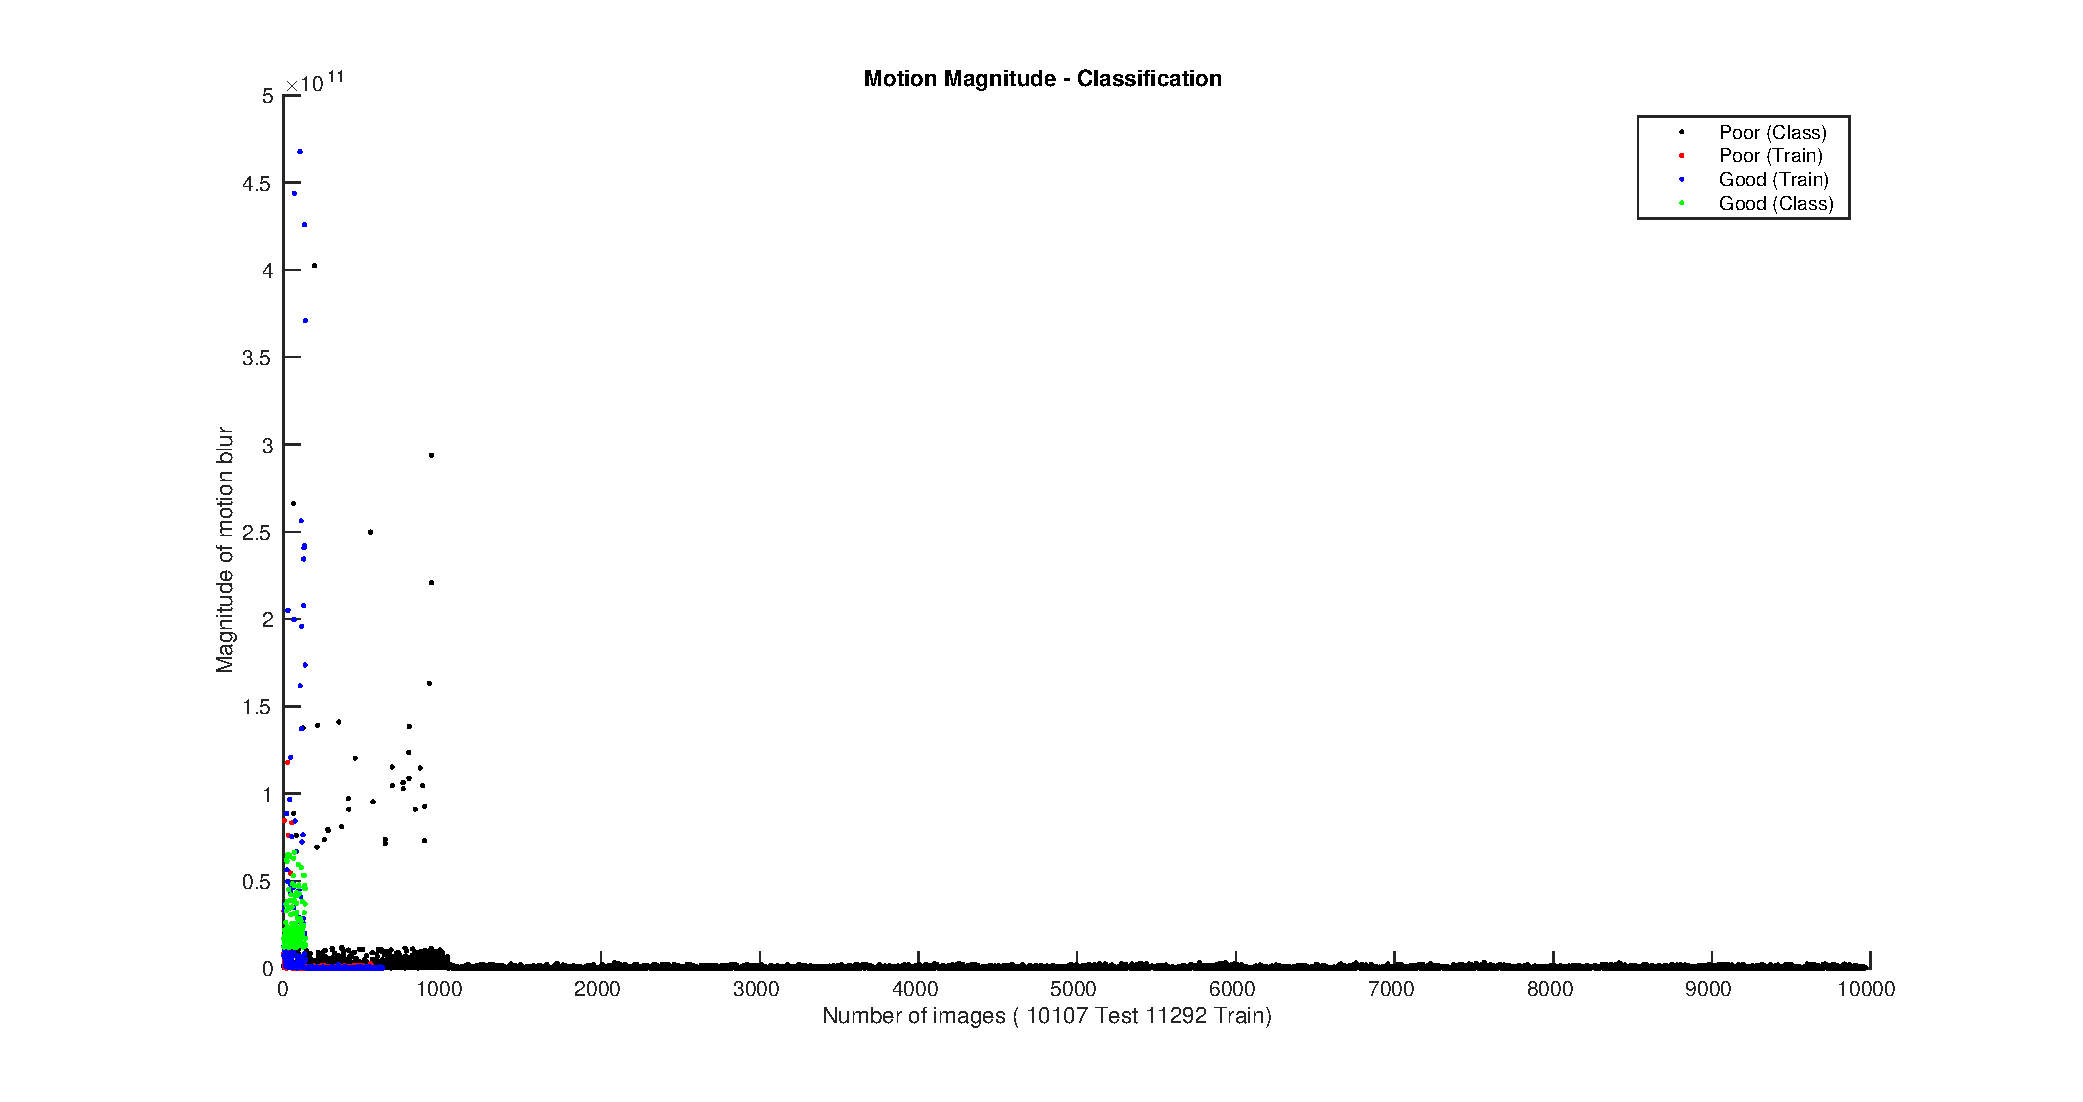
\includegraphics[width=0.9\linewidth, height=1.6cm]{pics/iqa_clas_motion}
		\caption{Res. of class. using IQA motion}
		\label{fig:clas_mot}
	\end{minipage}
	\begin{minipage}{0.48\linewidth}
		\centering
		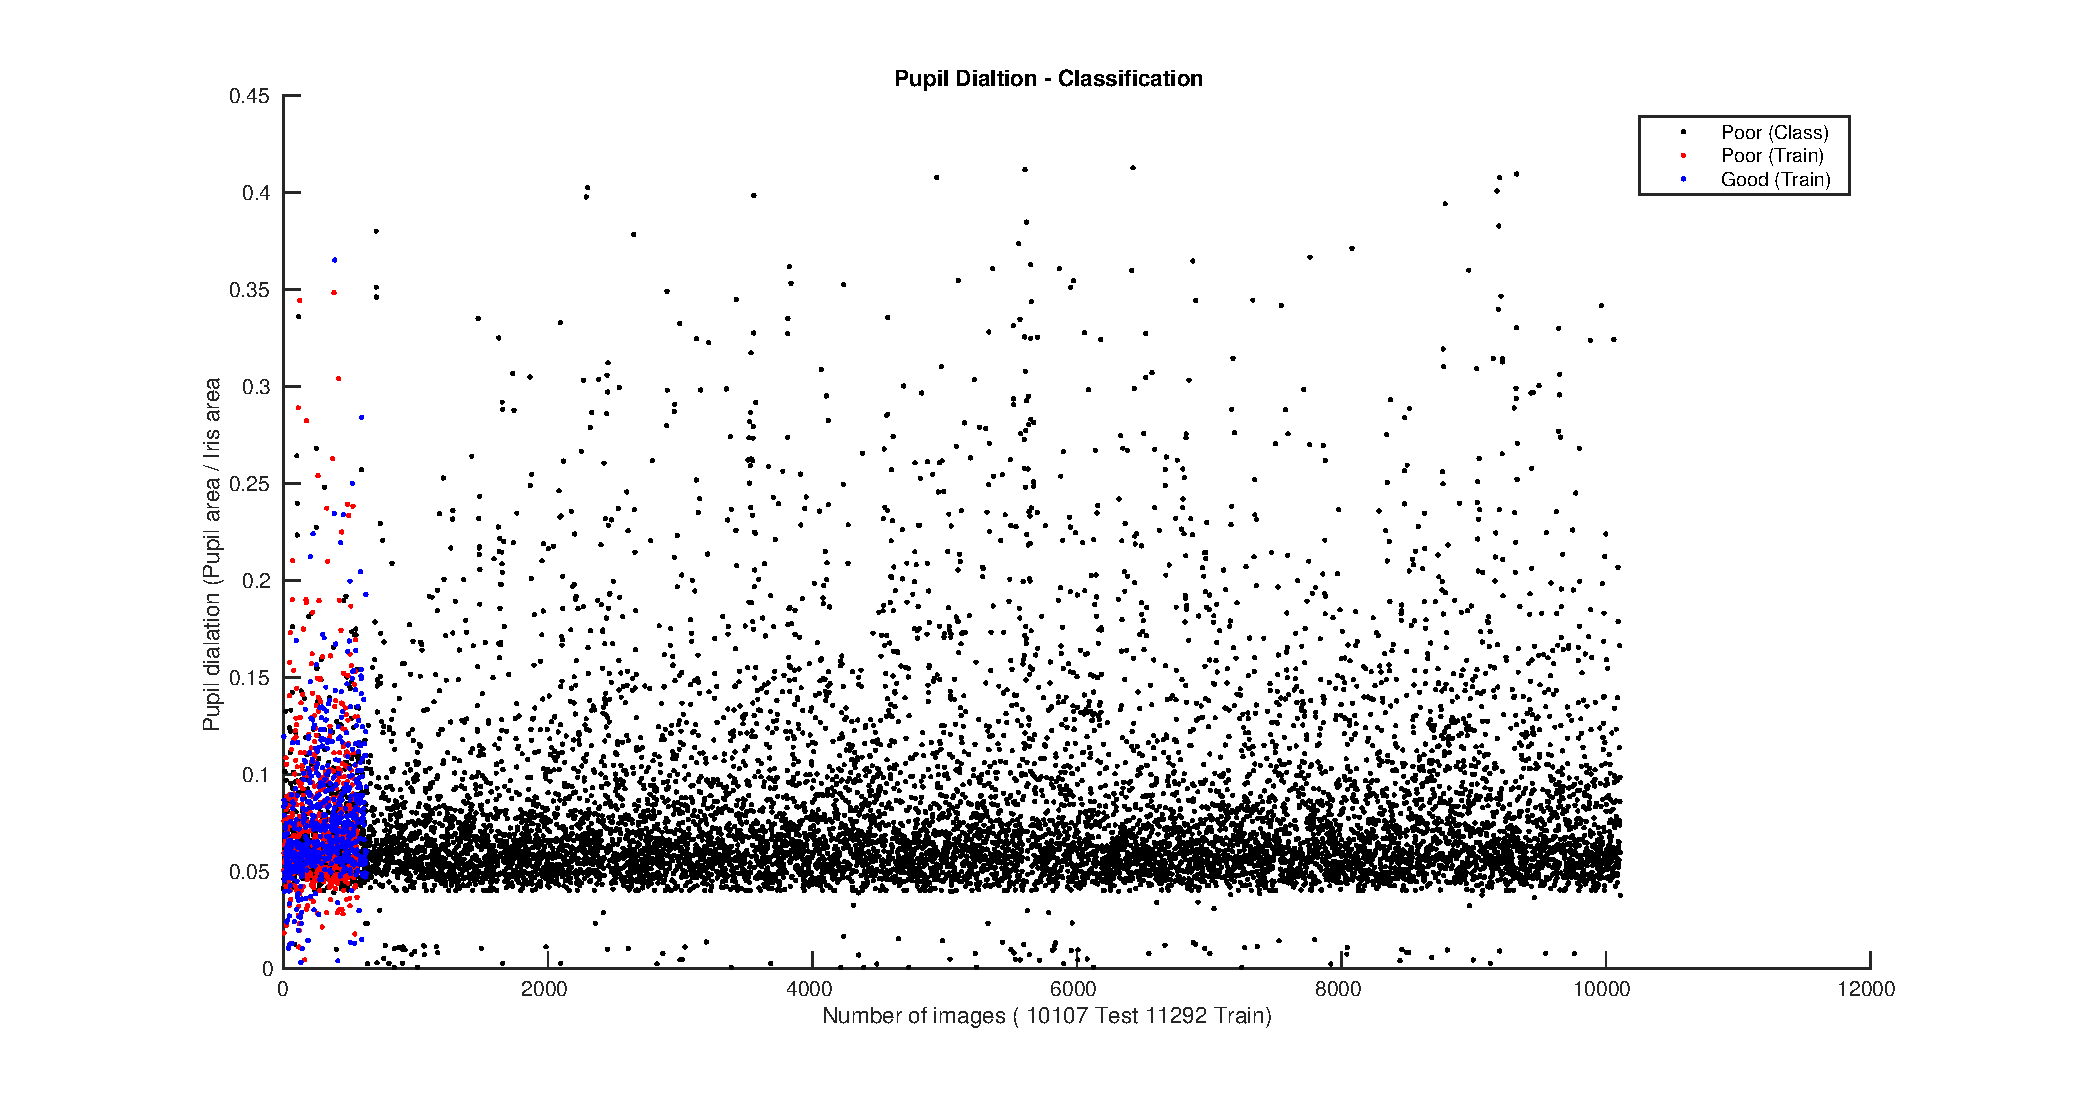
\includegraphics[width=0.9\linewidth, height=1.6cm]{pics/iqa_clas_pup_dial}
		\caption{Res. of class. using IQA pupil dilation}
		\label{fig:clas_pd}
	\end{minipage}
	\hfill
	\begin{minipage}{0.48\linewidth}
		\centering
		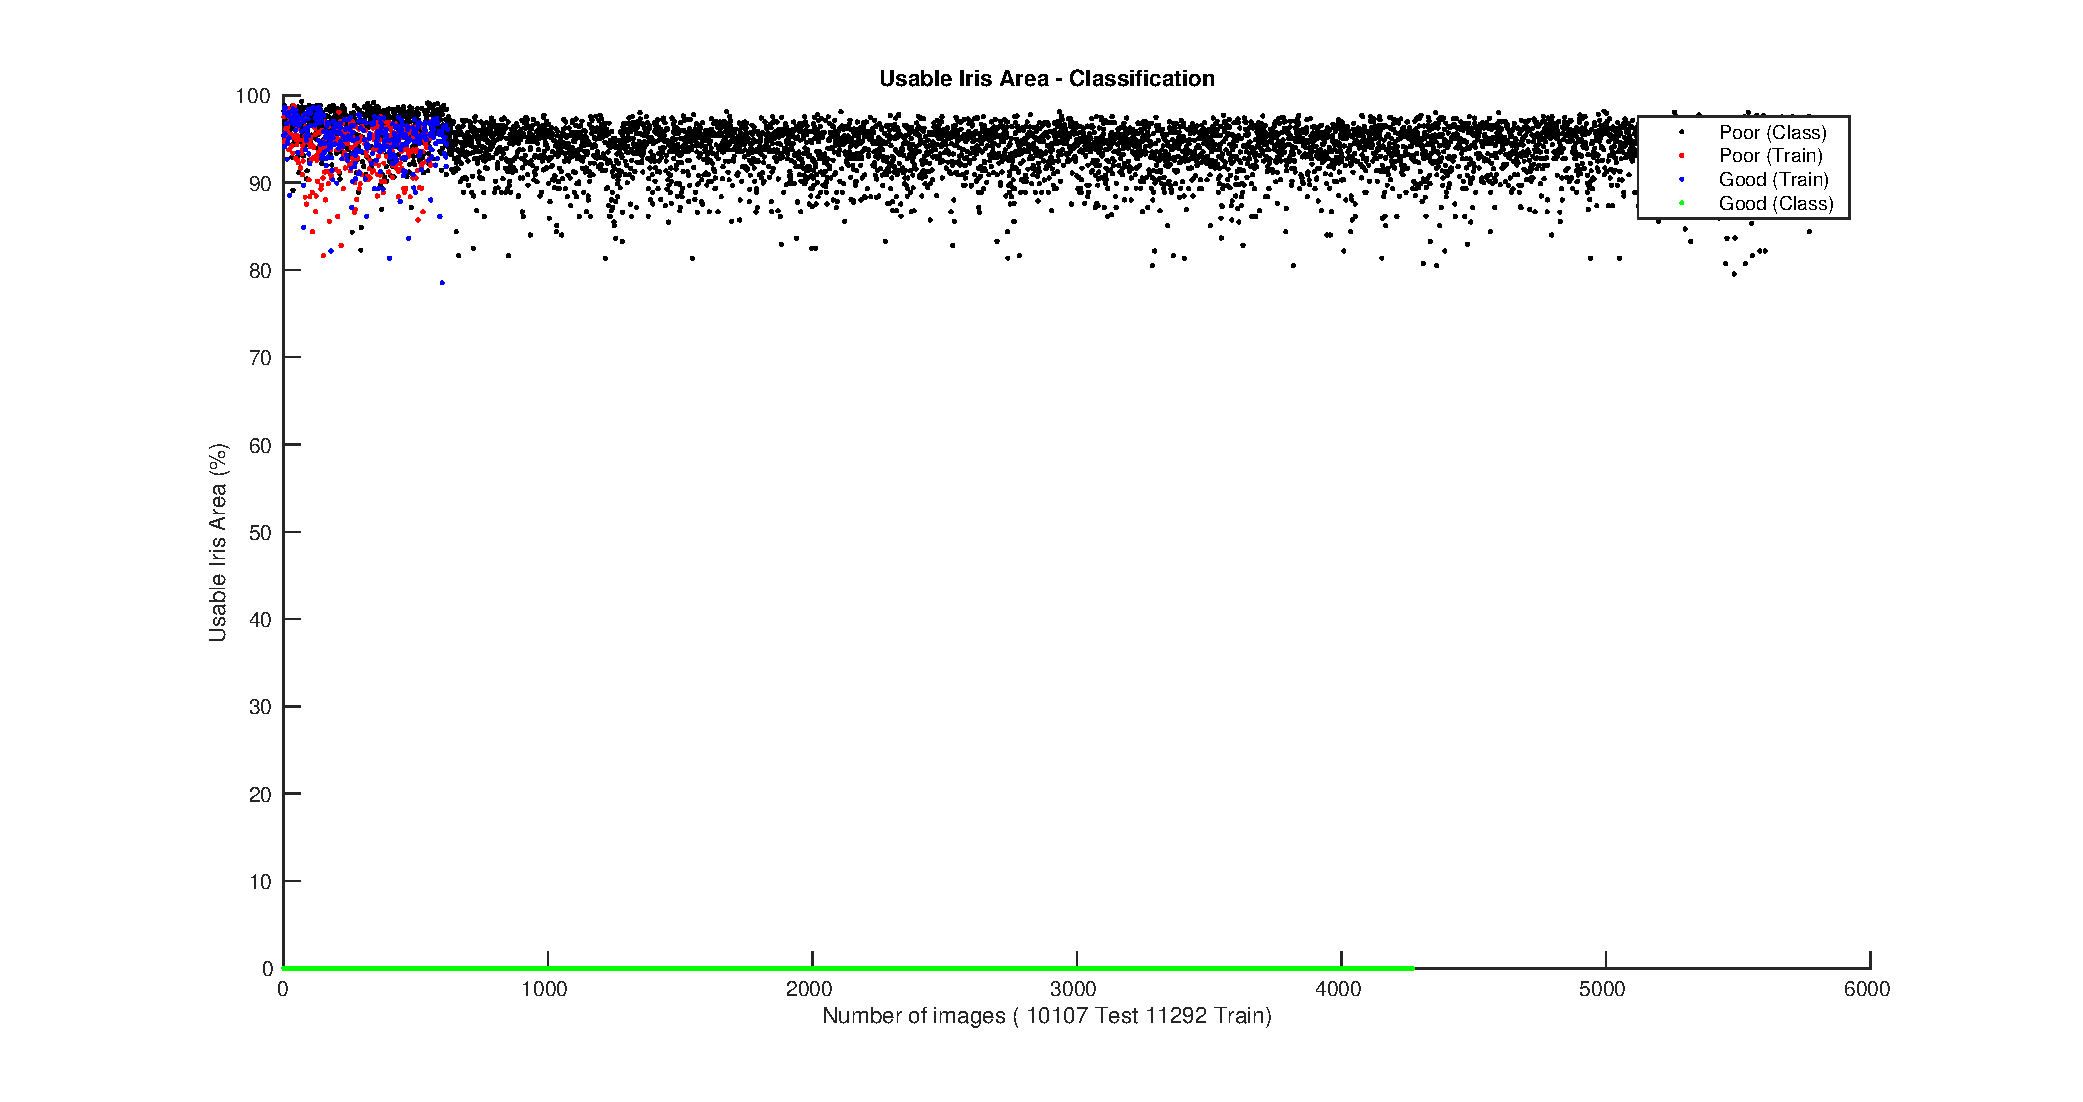
\includegraphics[width=0.9\linewidth, height=1.6cm]{pics/iqa_clas_usable_area}
		\caption{Res. of class. using BIQA UIA}
		\label{fig:clas_ua}
	\end{minipage}
	\begin{minipage}{0.48\linewidth}
		\centering
		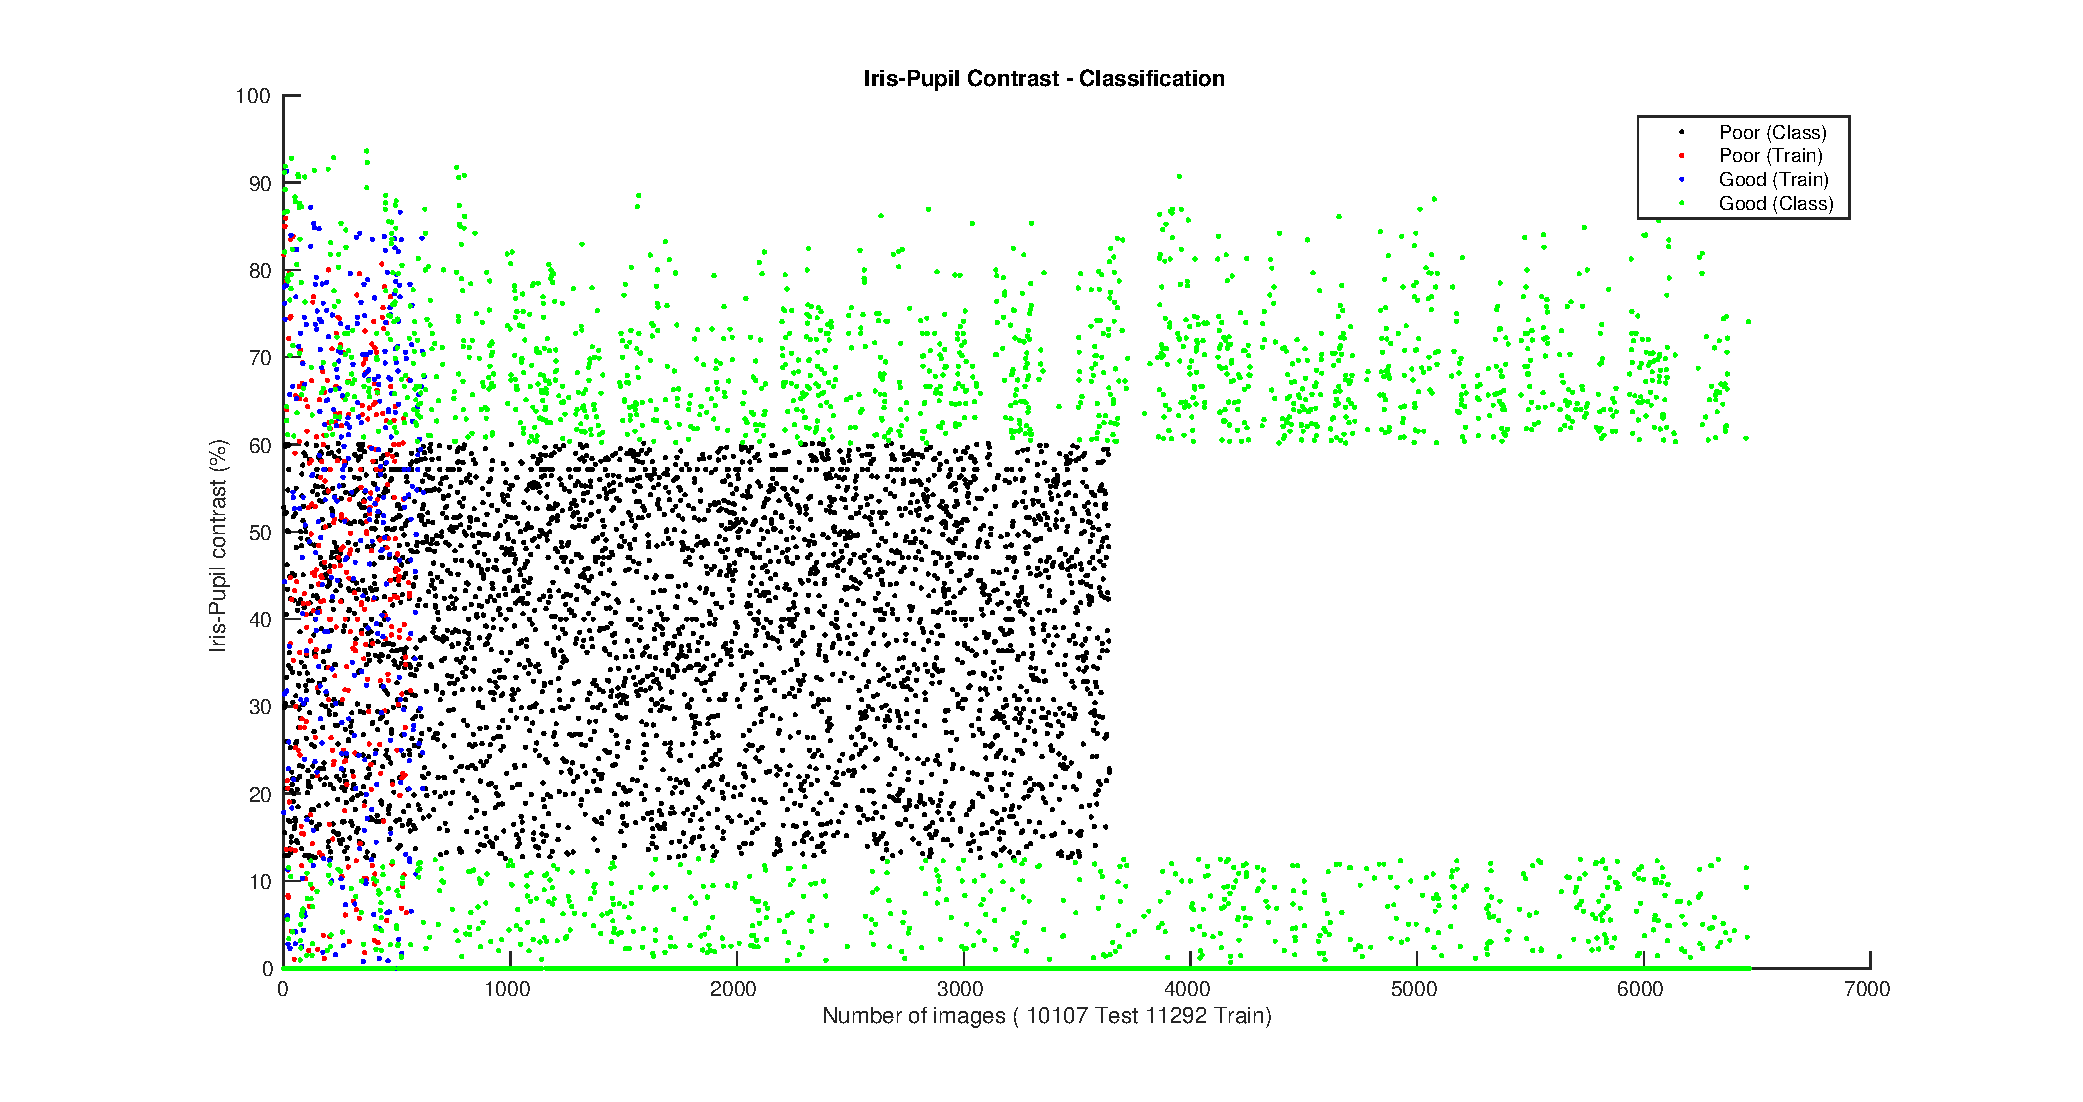
\includegraphics[width=0.9\linewidth, height=1.6cm]{pics/biqa_clas_ipc}
		\caption{Res. of class. using BIQA IPC}
		\label{fig:clas_ipc}
	\end{minipage}
	\hfill
	\begin{minipage}{0.48\linewidth}
		\centering
		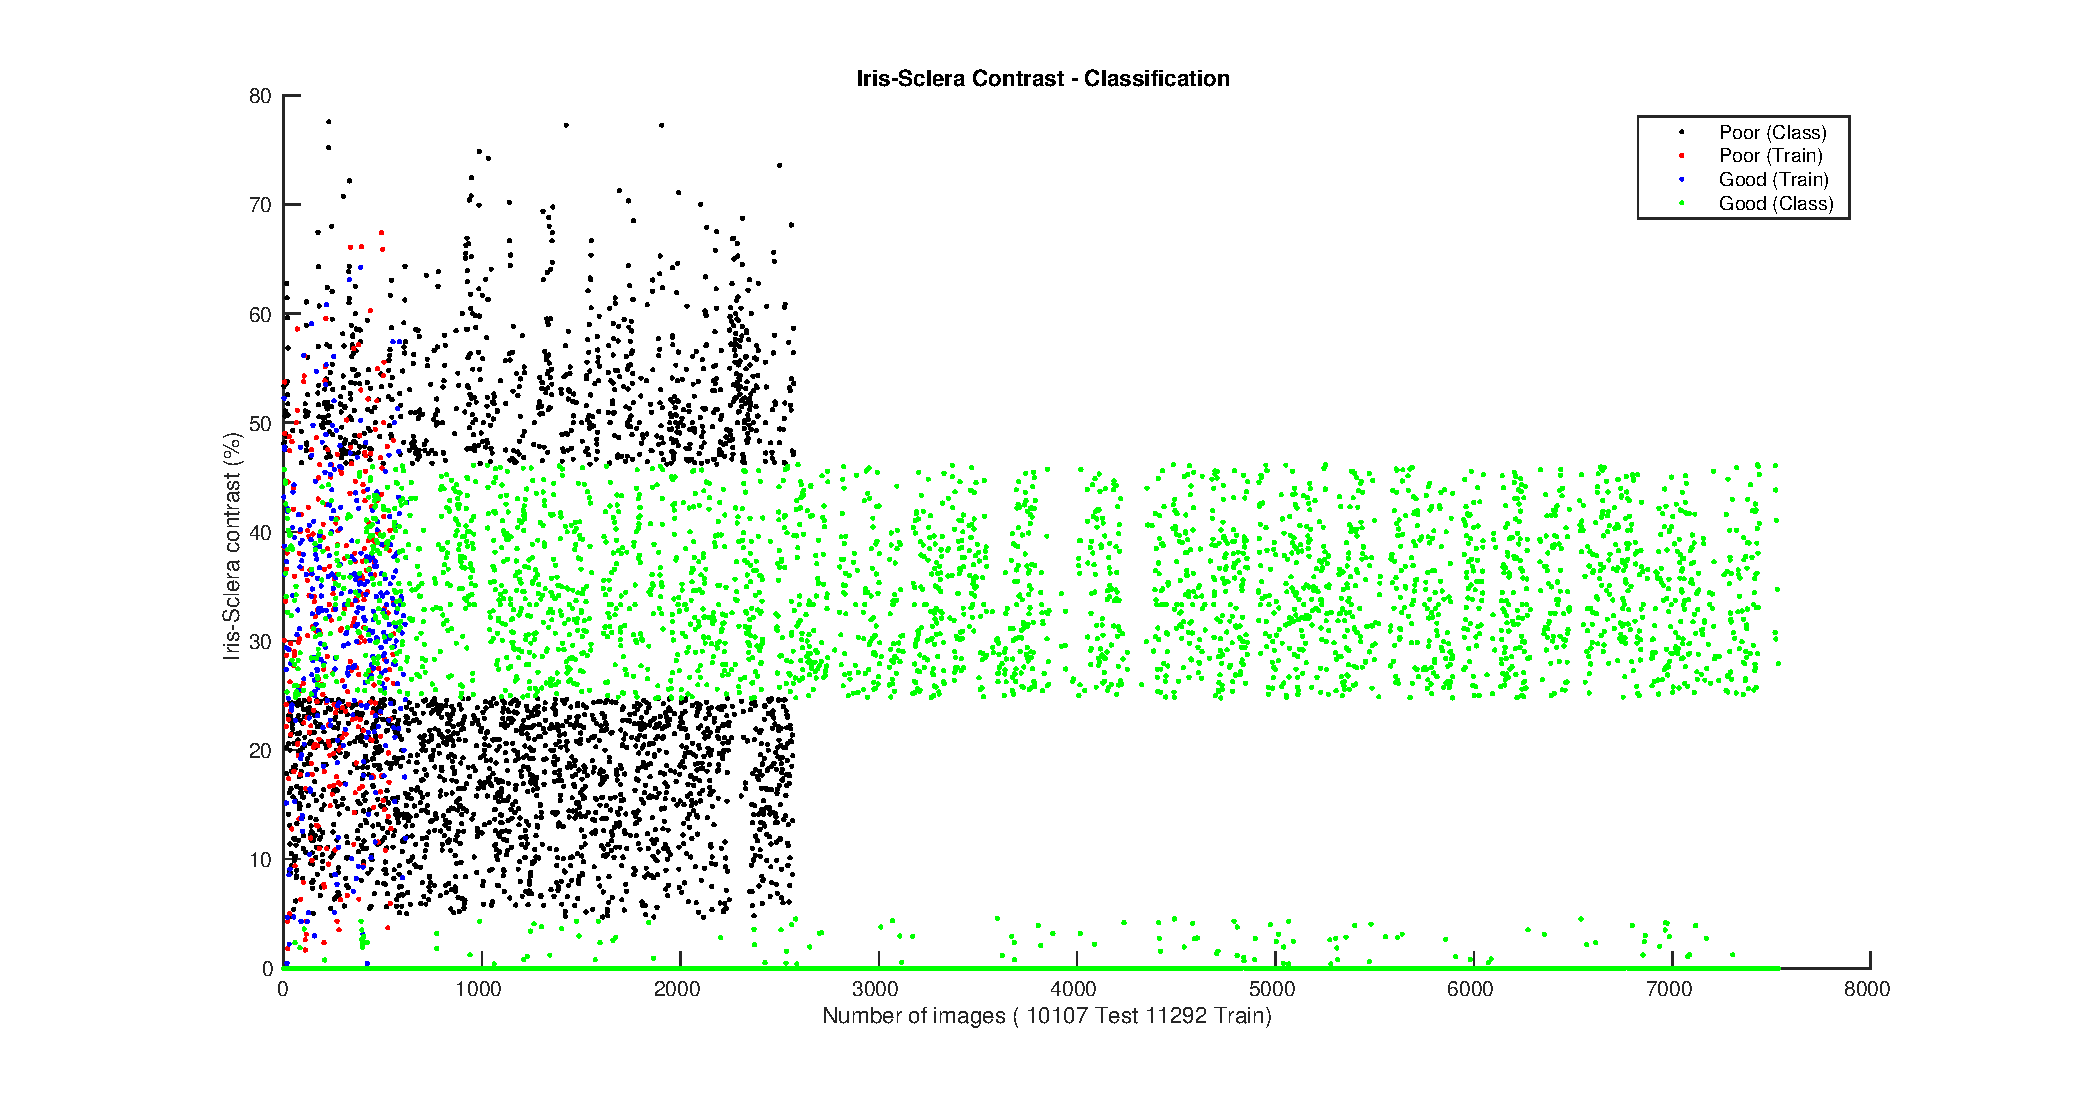
\includegraphics[width=0.9\linewidth, height=1.6cm]{pics/biqa_clas_isc}
		\caption{Res. of class. using BIQA ISC}
		\label{fig:clas_isc}
	\end{minipage}
	\begin{minipage}{0.48\linewidth}
		\centering
		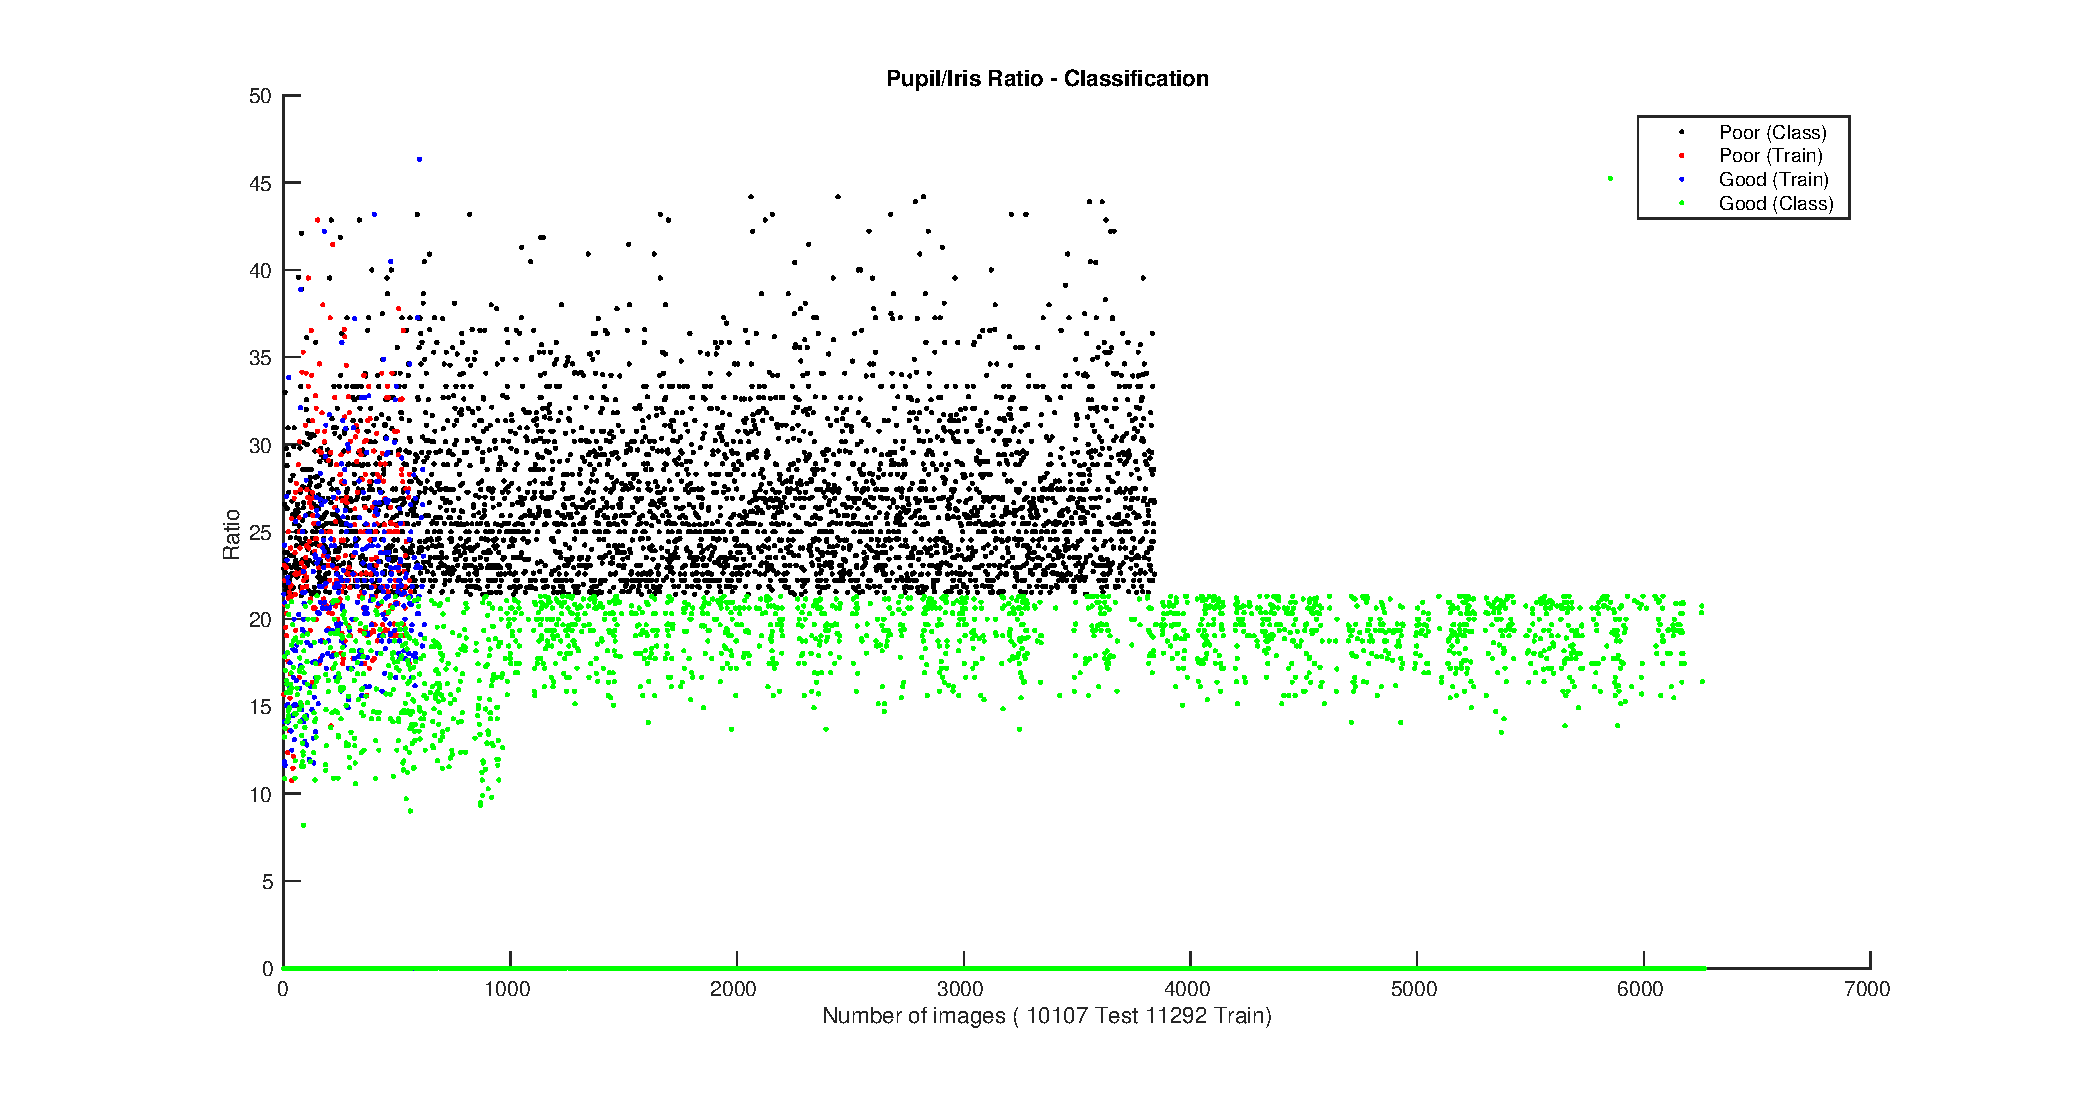
\includegraphics[width=0.9\linewidth, height=1.6cm]{pics/biqa_clas_pir}
		\caption{Res. of class. using BIQA pupil-iris rat.}
		\label{fig:clas_pir}
	\end{minipage}
	\hfill
	\begin{minipage}{0.48\linewidth}
		\centering
		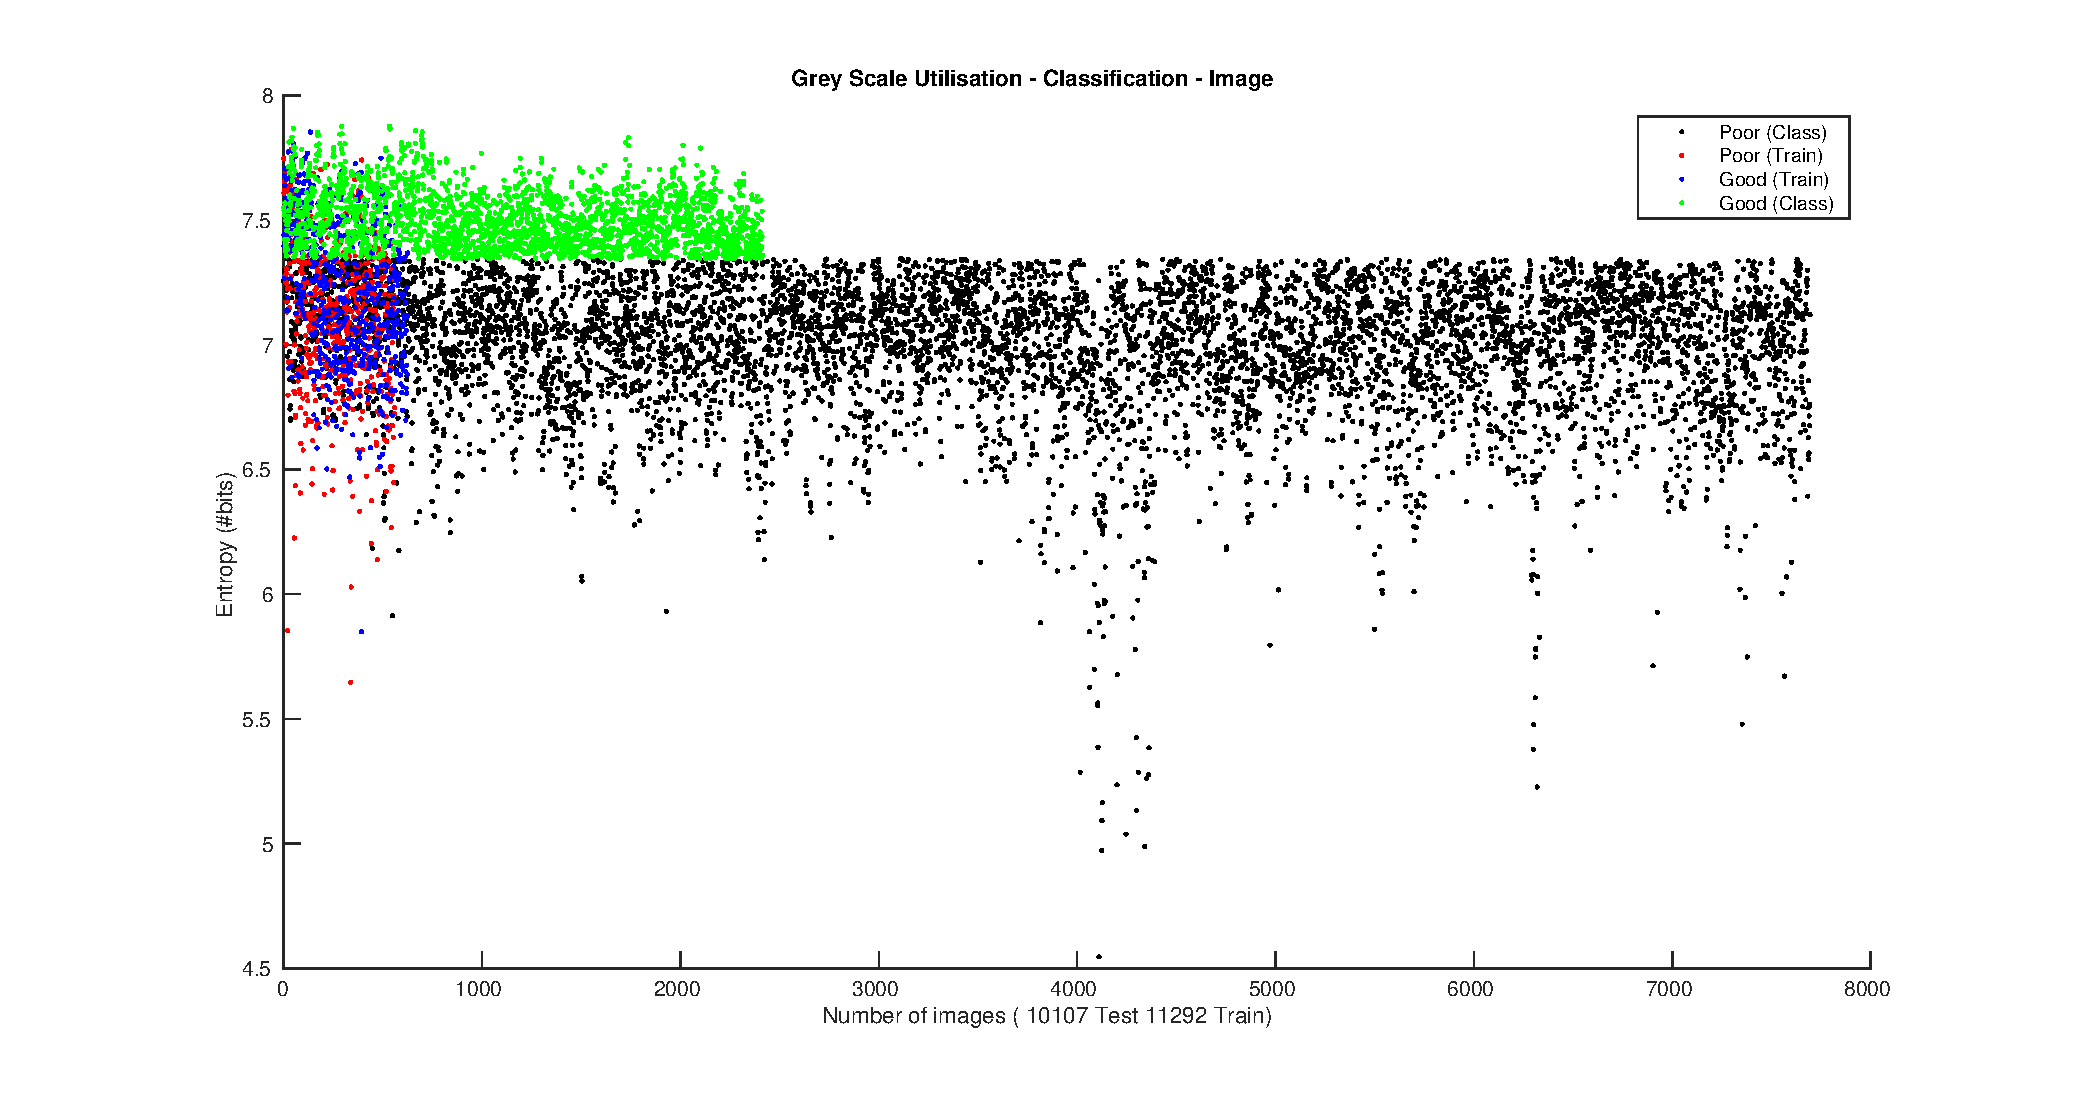
\includegraphics[width=0.9\linewidth, height=1.6cm]{pics/biqa_clas_gsu}
		\caption{Res. of class. using BIQA GSU}
		\label{fig:clas_gsu}
	\end{minipage}
\end{figure}
\begin{figure}
	\begin{minipage}{0.48\linewidth}
		\centering
		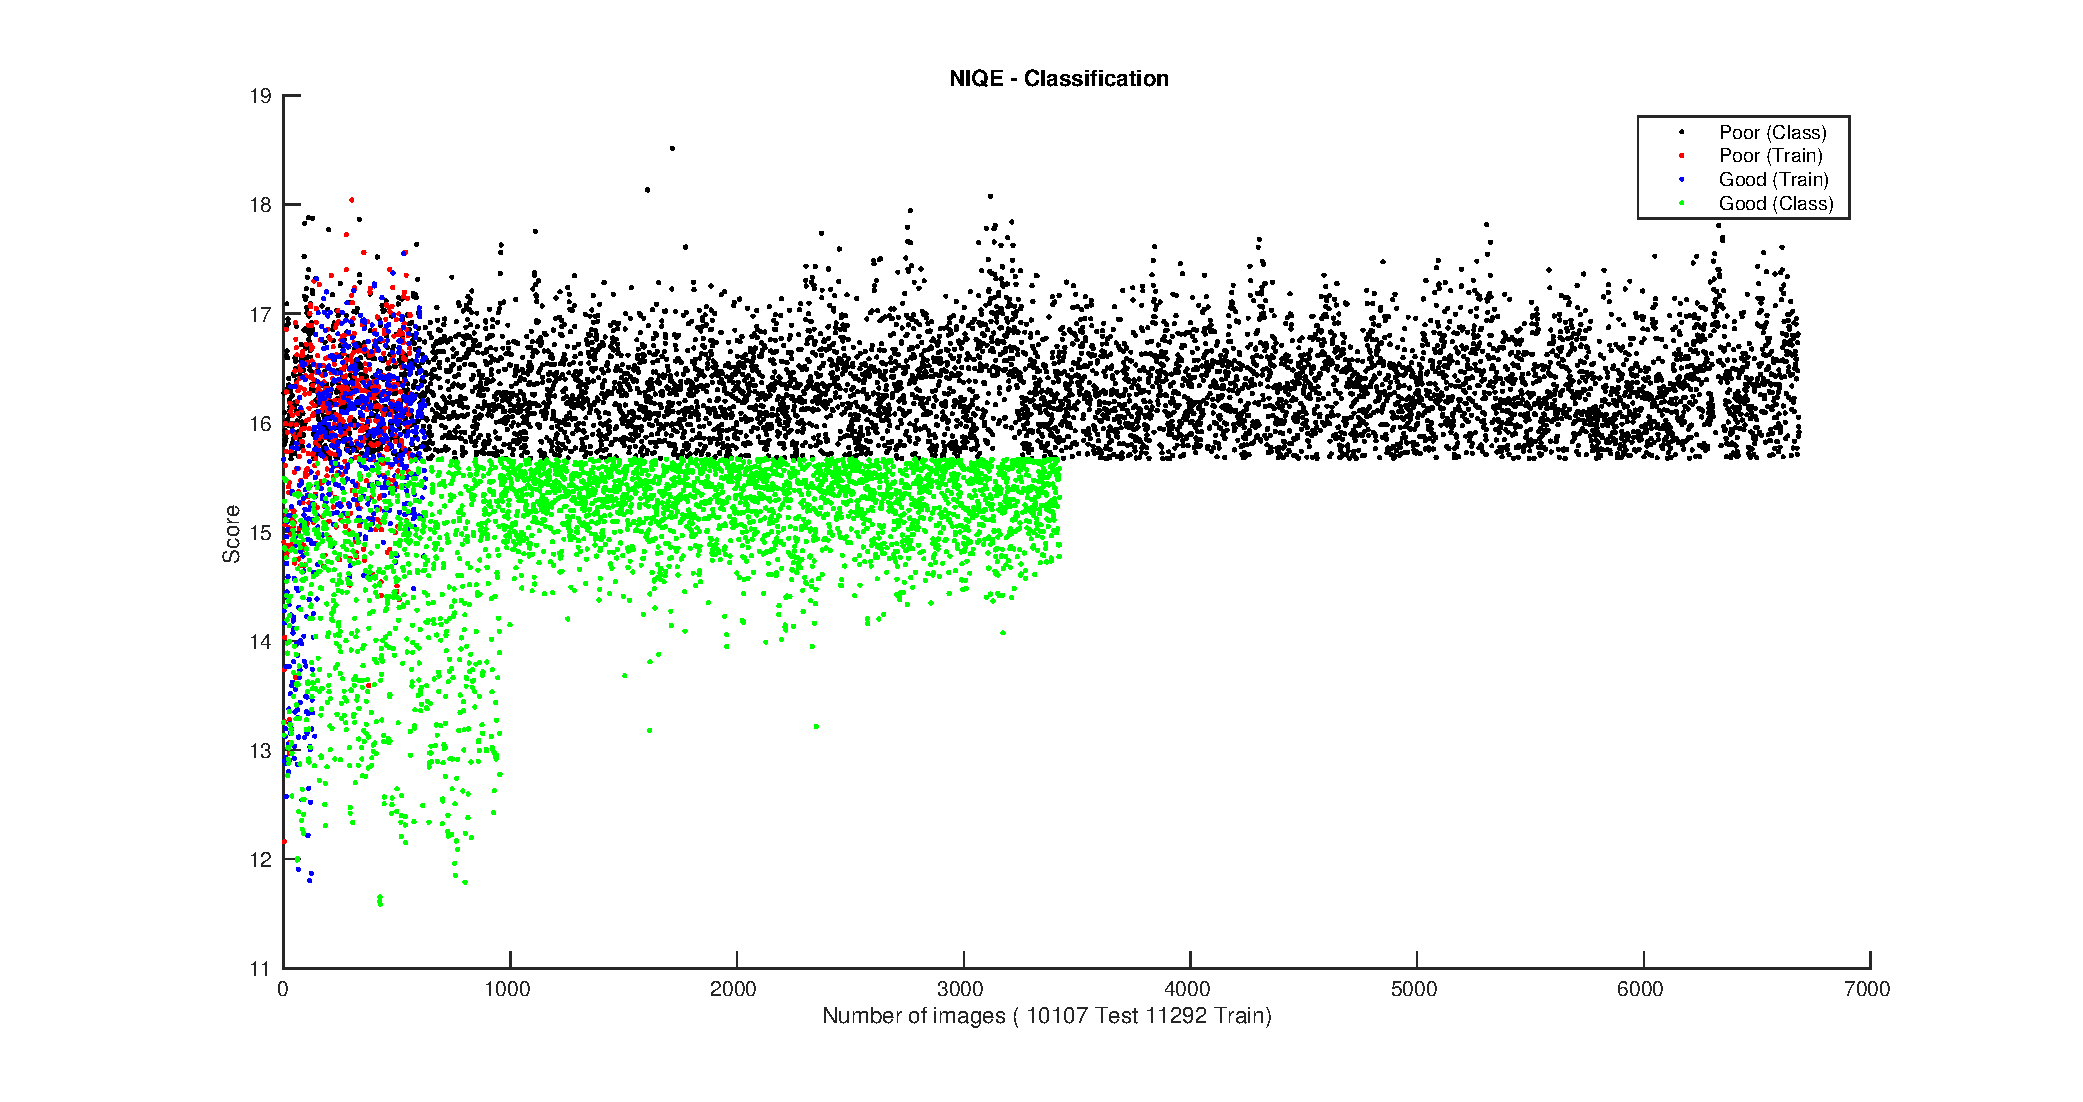
\includegraphics[width=0.9\linewidth, height=1.6cm]{pics/biqa_clas_niqe}
		\caption{Res. of class. using BIQA NIQE}
		\label{fig:clas_niqe}
	\end{minipage}
	\hfill
	\begin{minipage}{0.48\linewidth}
		\centering
		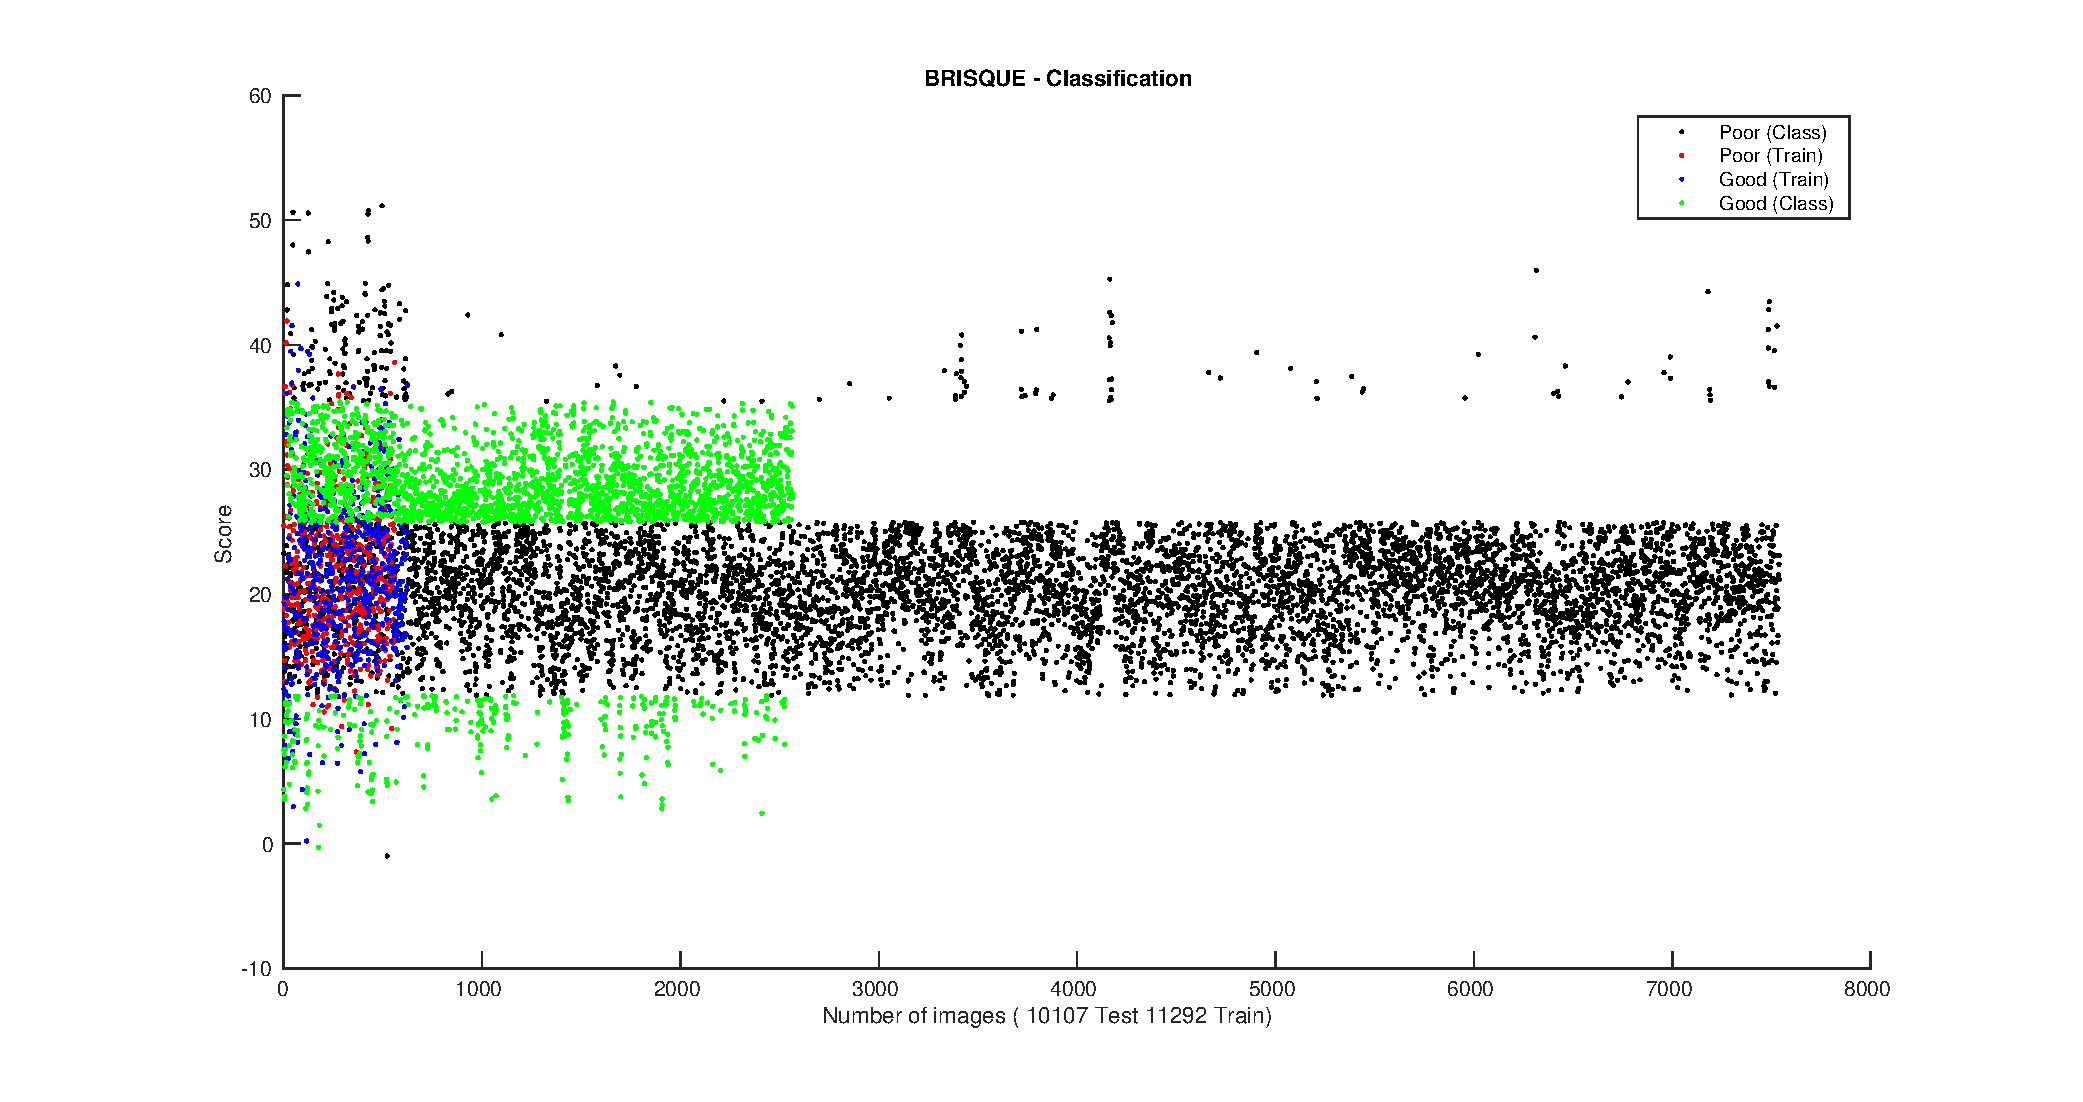
\includegraphics[width=0.9\linewidth, height=1.6cm]{pics/biqa_clas_brisque}
		\caption{Res. of class. using BIQA BRISQUE}
		\label{fig:clas_brisque}
	\end{minipage}
\end{figure}
\begin{figure}
	\begin{minipage}{0.48\linewidth}
		\centering
		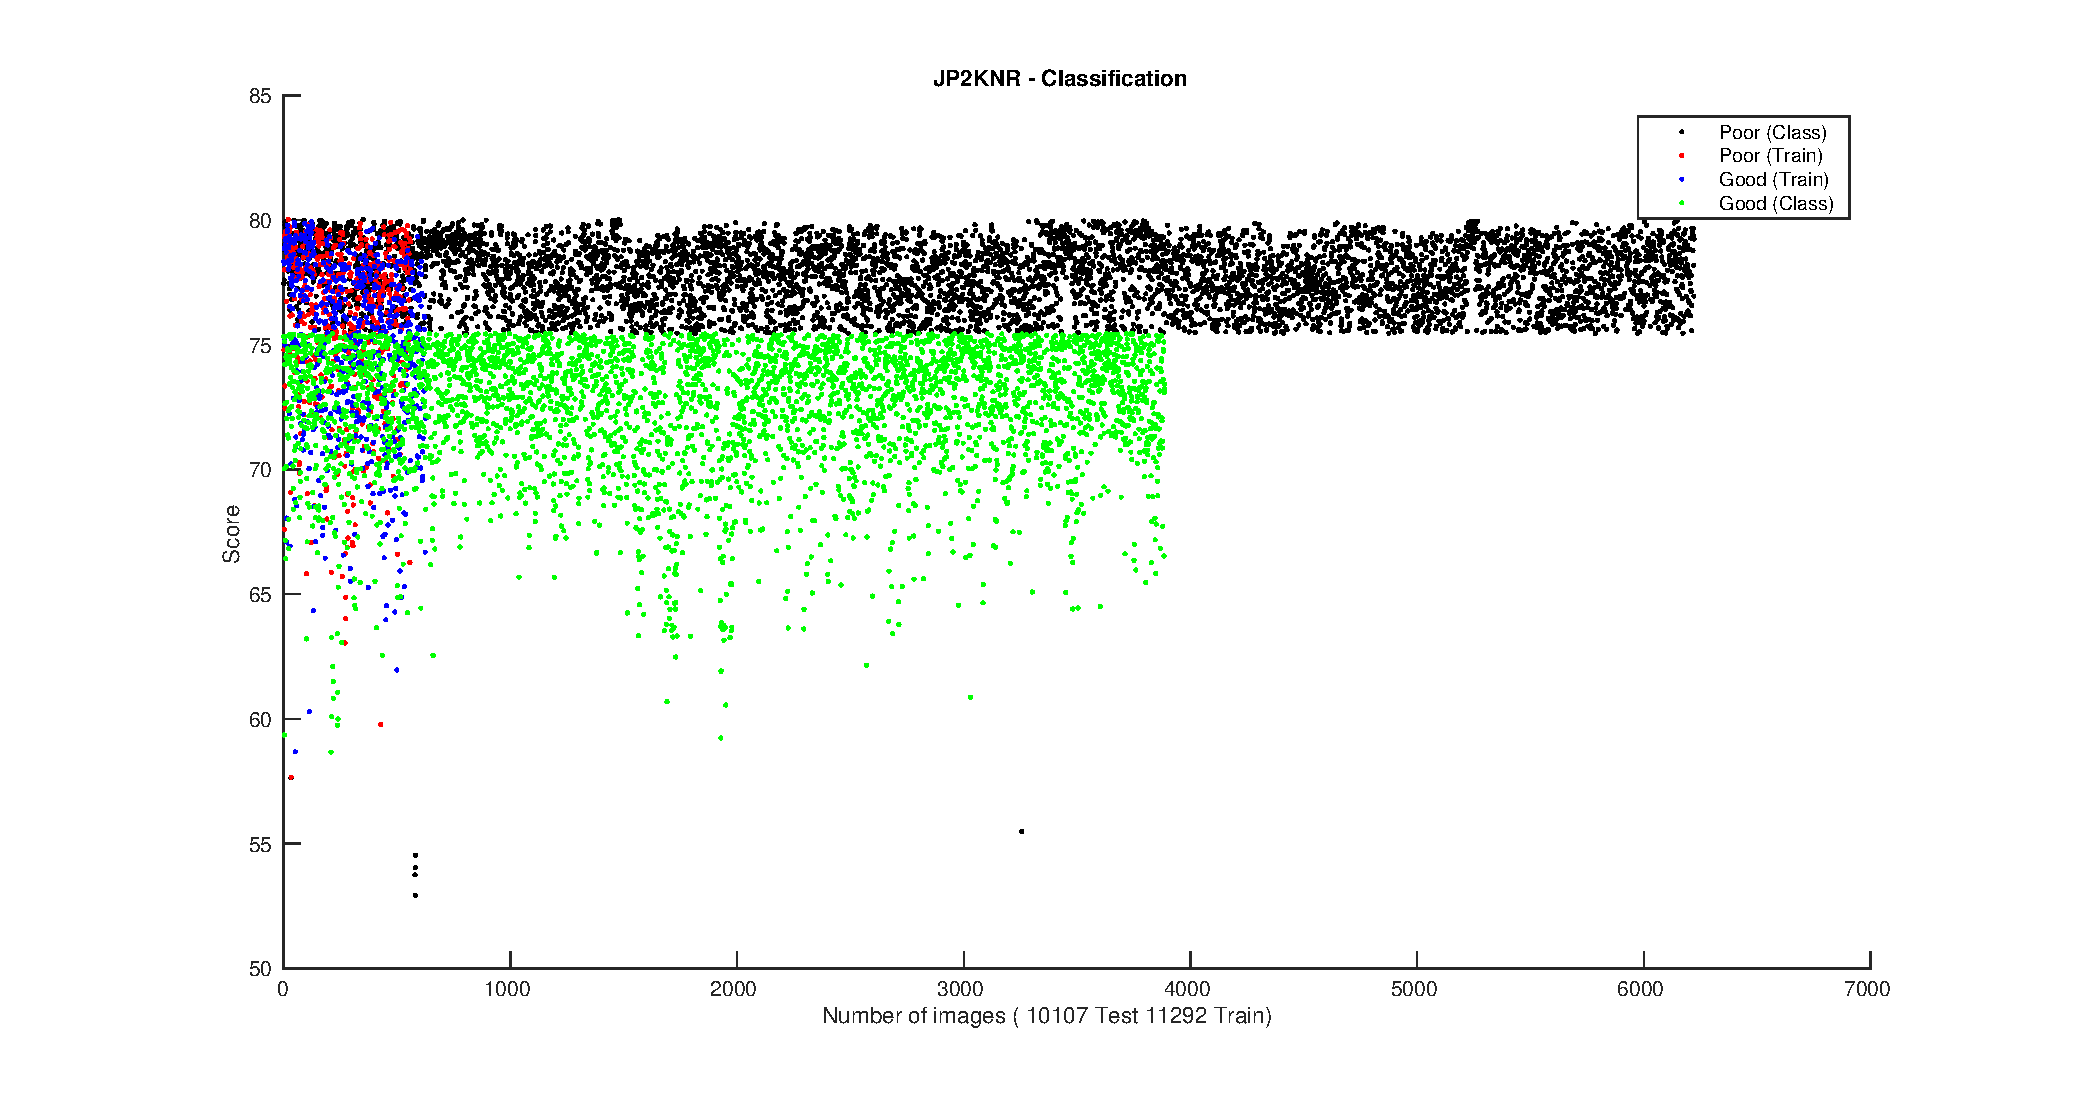
\includegraphics[width=0.9\linewidth, height=1.6cm]{pics/biqa_clas_jp2knr}
		\caption{Res. of class. using BIQA JP2KNR}
		\label{fig:clas_jp2knr}
	\end{minipage}
	\hfill
	\begin{minipage}{0.48\linewidth}
		\centering
		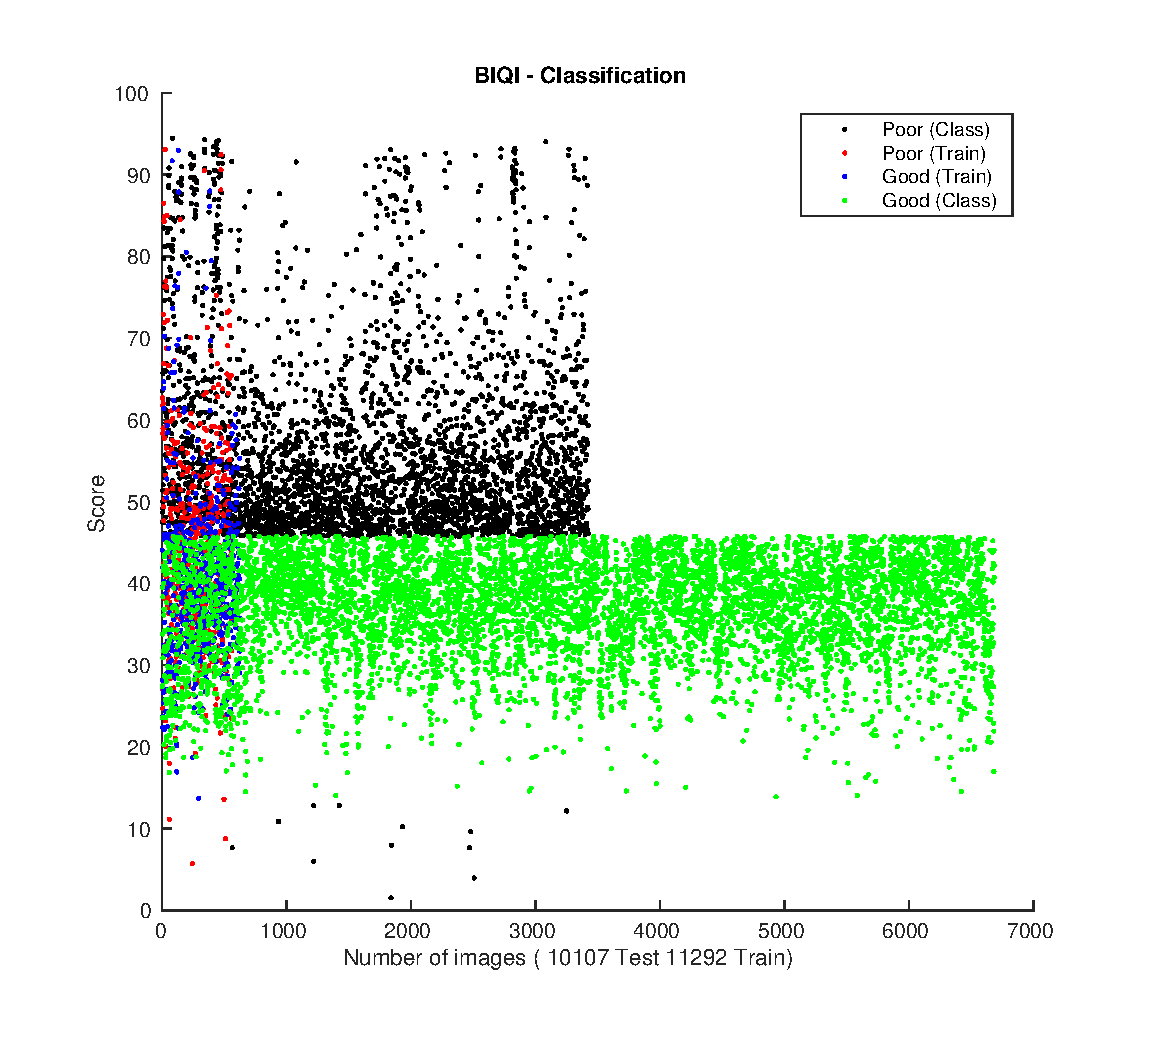
\includegraphics[width=0.9\linewidth, height=1.6cm]{pics/biqa_clas_biqi}
		\caption{Res. of class. using BIQA BIQI}
		\label{fig:clas_biqi}
	\end{minipage}
\end{figure}
\pagebreak


